\documentclass[12pt,a4paper,oneside]{memoir}
%\documentclass[titlepage,12pt,a4paper]{book}

% substituir linha seguinte por 
\usepackage[english]{babel} 
% se o relatório for escrito na língua inglesa.
%\usepackage[portuguese]{babel}

% \usepackage[utf8]{inputenc}
\usepackage[T1]{fontenc}
\usepackage{float}
\usepackage{makeidx}
\usepackage{xspace}
\usepackage{graphicx,color,times}
\usepackage{fancyhdr}
% \usepackage{pxfonts}
% \usepackage{times}
% \usepackage{mathptm}
% \usepackage{amssymb}
% \usepackage{amsfonts}

\usepackage{amsmath}
\usepackage{latexsym}
\usepackage[printonlyused]{acronym}
\usepackage{float}
\usepackage{listings}
\usepackage{tocbibind}
\usepackage{natbib}
\usepackage{hyperref}
\usepackage{caption}

% \usepackage{glossaries}
% \makeglossaries

% \renewcommand{\ttdefault}{phv}

\pagestyle{fancy}
\renewcommand{\chaptermark}[1]{\markboth{#1}{}}
\renewcommand{\sectionmark}[1]{\markright{\thesection\ #1}}
\fancyhf{} \fancyhead[LE,RO]{\bfseries\thepage}
\fancyhead[LO]{\bfseries\rightmark}
\fancyhead[RE]{\bfseries\leftmark}
\renewcommand{\headrulewidth}{0.5pt}
\renewcommand{\footrulewidth}{0pt}
\setlength{\headheight}{15.6pt}
\setlength{\marginparsep}{0cm}
\setlength{\marginparwidth}{0cm}
\setlength{\marginparpush}{0cm}
\addtolength{\hoffset}{-1.0cm}
\addtolength{\oddsidemargin}{\evensidemargin}
\addtolength{\oddsidemargin}{0.5cm}
\addtolength{\evensidemargin}{-0.5cm}


\usepackage{fix-cm}
\usepackage{fourier}
\usepackage[scaled=.92]{helvet}
\definecolor{ChapGrey}{rgb}{0.6,0.6,0.6}
\newcommand{\LargeFont}{
  \usefont{\encodingdefault}{\rmdefault}{b}{n}
  \fontsize{60}{80}\selectfont\color{ChapGrey}
  }
\makeatletter
\makechapterstyle{GreyNum}{
  \renewcommand{\chapnamefont}{\large\sffamily\bfseries\itshape}
  \renewcommand{\chapnumfont}{\LargeFont}
  \renewcommand{\chaptitlefont}{\Huge\sffamily\bfseries\itshape}
  \setlength{\beforechapskip}{0pt}
  \setlength{\midchapskip}{40pt}
  \setlength{\afterchapskip}{60pt}
  \renewcommand\chapterheadstart{\vspace*{\beforechapskip}}
  \renewcommand\printchaptername{
  \begin{tabular}{@{}c@{}}
    \chapnamefont \@chapapp\\}
    \renewcommand\chapternamenum{\noalign{\vskip 2ex}}
    \renewcommand\printchapternum{\chapnumfont\thechapter\par}
    \renewcommand\afterchapternum{
  \end{tabular}
  \par\nobreak\vskip\midchapskip}
  \renewcommand\printchapternonum{}
  \renewcommand\printchaptertitle[1]{
  {\chaptitlefont{##1}\par}}
  \renewcommand\afterchaptertitle{\par\nobreak\vskip \afterchapskip}
}
\makeatother
\chapterstyle{GreyNum}

\setcounter{tocdepth}{3}
\setsecnumdepth{subsubsection}

\renewcommand{\ttdefault}{lmtt}


% NEW COLORS
\definecolor{dark}{gray}{0.25}
\definecolor{lgray}{gray}{0.9}
\definecolor{dkblue}{rgb}{0,0.13,0.4}
\definecolor{dkgreen}{rgb}{0,0.6,0}
\definecolor{gray}{rgb}{0.5,0.5,0.5}
\definecolor{mauve}{rgb}{0.58,0,0.82}

\lstset{ %
  language=C,                    basicstyle=\footnotesize,
  numbers=none,                  numberstyle=\tiny\color{gray}, 
  stepnumber=1,                  numbersep=5pt,
  backgroundcolor=\color{white}, showspaces=false,
  showstringspaces=false,        showtabs=false,
  frame=single,                  rulecolor=\color{black},
  tabsize=2,                     captionpos=b,
  breaklines=true,               breakatwhitespace=false,
  title=\lstname,                keywordstyle=\color{blue},
  commentstyle=\color{dkgreen},  stringstyle=\color{mauve},
  escapeinside={\%*}{*)},        morekeywords={*},
  belowskip=0cm
}

\renewcommand{\lstlistingname}{Excerto de Código}
\renewcommand{\lstlistlistingname}{Lista de Excertos de Código}

\renewcommand{\today}{\day \ifcase \month \or January\or February\or March\or %
April \or May \or June \or July \or August\or September \or October \or November\or %
December\fi of \number \year} 




\begin{document}

%Capa

\thispagestyle{empty}
\setcounter{page}{-1}

\begin{center}
\begin{Huge}
\textbf{University of Beira Interior}
\end{Huge}
\end{center}

\begin{center}
\begin{Huge}
Department of Computer Science
\end{Huge}
\end{center}

\vspace{0,07cm}
\begin{figure}[!htb]
\centering

\includegraphics[width=191pt]{ubi-fe-di.png}
\end{figure}

\vspace{0.5cm}
\begin{center}
\begin{Large}
\textbf{\emph{04 - Use of Generative Adversarial Networks
(GANs) to build Interpretable and Intelligent Recognition Systems}}
\end{Large}
\end{center}


\vspace{0.5cm}
\begin{center}
\begin{normalsize}
\begin{large}
Written by :
\end{large}
\end{normalsize}
\end{center}

\vspace{0.2cm}
\begin{center}
\begin{large}
\textbf{Pedro Jorge Franco Brito}
\end{large}
\end{center}

\vspace{0,5cm}
\begin{center}
\begin{normalsize}
\begin{large}
Supervisor:
\end{large}
\end{normalsize}
\end{center}

\vspace{0.2cm}
\begin{center}
\begin{large}
\textbf{Professor Dr. Hugo Pedro Proença}
\end{large}
\end{center}



\vspace{0.5cm}
\begin{center}
\begin{normalsize}
\today
\end{normalsize}
\end{center}


%Capa
\clearpage{\thispagestyle{empty}\cleardoublepage}

\frontmatter

\chapter*{Acknowledgements}
\label{chap:ack}

I would first, like to thank Professor Hugo Proença immensely for always being available to help me and for all the support he gave me throughout the development of this project. I would also like to thank my parents for always staying by my side and supporting me in every choice of my life.

\clearpage{\thispagestyle{empty}\cleardoublepage}


\tableofcontents

\clearpage{\thispagestyle{empty}\cleardoublepage}

\listoffigures

% Se não existirem tabelas, comentar as seguintes linhas
%\clearpage{\thispagestyle{empty}\cleardoublepage}
\listoftables

% Se existirem trechos de código, descomentar as seguintes linhas
% \clearpage{\thispagestyle{empty}\cleardoublepage}
% \lstlistoflistings

\clearpage{\thispagestyle{empty}\cleardoublepage}
\chapter*{Acronyms}
\label{chap:acro}

\begin{acronym}[CGAN]
  \acro{CGAN}{\emph{Conditional Generative Adversarial Networks}}
\end{acronym}

\begin{acronym}[GAN]
  \acro{GAN}{\emph{Generative Adversarial Networks}}
\end{acronym}


\begin{acronym}[CPU]
  \acro{CPU}{\emph{Central Processing Unit }}
\end{acronym}


\begin{acronym}[IDE]
  \acro{IDE}{\emph{Integrated Development Environment }}
\end{acronym}

\begin{acronym}[MLP]
  \acro{MLP}{\emph{Multilayer Perceptron}}
\end{acronym}


% \clearpage{\pagestyle{empty}\cleardoublepage}
% \chapter*{Glossário}
\makeglossaries

\newglossaryentry{.NET Framework}
{
  name={.NET Framework},
  description={É uma plataforma para desenvolvimento e funcionamento de aplicações desenvolvida pela Microsoft.}
}

\newglossaryentry{ASP.NET}
{
  name={ASP .Net},
  description={É uma plataforma da Microsoft para o desenvolvimento de aplicações Web e é o sucessor da tecnologia ASP.}
}

\newglossaryentry{CS}
{
  name={C\#},
  description={Lê-se \textit{C Sharp} e é uma linguagem de programação orientada a objectos, desenvolvida pela Microsoft, inicialmente para a plataforma .NET. O C\# é inspirado na junção entre as linguagens C++ e Java.}
}


\newglossaryentry{Java}
{
  name={JAVA},
  description={É uma linguagem de programação orientada a objectos, desenvolvida pela Sun Microsystems na década de 90. Hoje pertence à empresa Oracle.}
}


\newglossaryentry{OpenDMTP}
{
  name={OpenDMTP},
  description={\textit{Open Device Monitoring and Tracking Protocol} é um protocolo e uma \textit{framework} abertos que permite a comunicação bidireccional entre servidores e clientes através da internet.}
}


\newglossaryentry{OpenGTS}
{
  name={Open GTS},
  description={É o primeiro projecto \textit{Open Source} \textit{Web-Based} para controlo de frotas por GPS.}
}


\newglossaryentry{VS2010}
{
  name={Visual Studio 2010},
  description={\textit{Microsoft Visual Studio 2010} é um sistema de desenvolvimento desenvolvido pela Microsoft e é dedicado ao Framework .NET, que contem um conjunto de ferramentas de desenvolvimento projectadas para auxiliar os programadores a enfrentarem desafios complexos.}
}


\newglossaryentry{WebS}
{
	name={Web Service},
	description={Web services são aplicações modulares auto-descritas e auto-contidas, que permitem a integração de sistemas e a comunicação entre aplicações de diferentes tipos.}
}


\newglossaryentry{WebBased}
{
	name={Web Based},
	description={Aplicação desenvolvida para a Web.}
}

\newglossaryentry{Roaming}
{
	name={Roaming},
	description={Define a possibilidade de um utilizador de uma determinada rede obter rede/conecção fora da área geográfica onde foi registado.}
}


\newglossaryentry{Smartphone}
{
	name={Smartphone},
	description={Smartphone é um telefone móvel que contem muitas das principais tecnologias de comunicação e serviços que existem nos computadores pessoais, como acesso a e-mails, serviços de mensagens instantâneas, internet, GPS, entre outros.}
}

\newglossaryentry{TCPIP}
{
	name={TCP/IP},
	description={É um conjunto de protocolos de comunicação entre computadores ligados rede. O nome TCP/IP surge da união entre dois protocolos: o TCP (Transmission Control Protocol) e o protocolo IP (Internet Protocol).}
}

\newglossaryentry{Firewall}
{
	name={Firewall},
	description={É o nome criado para definir um dispositivo para uma rede de computadores que tem como objectivo criar uma política de segurança num determinado ponto de controlo da rede.}
}

\newglossaryentry{JavaScript}
{
	name={JavaScript},
	description={É uma linguagem de programação baseada na linguagem de programação ECMAScript. Actualmente é a linguagem de programação mais utilizada em \textit{``Client-Side''} nos \textit{browsers}.}
}

\newglossaryentry{Flash}
{
	name={Flash},
	description={Desenvolvido pela Macromedia, o Flash é um software utilizado para criação de animações interactivas que funcionam incorporadas em \textit{Browsers}, \textit{Desktop}, \textit{Smartphones}, \textit{Tablets}, e Televisores.}
}


\newglossaryentry{StoredProcedure}
{
	name={Stored Procedure },
	description={É o nome dado a um conjunto de comandos numa base de dados de forma a simplificar a sua utilização.}
}

\newglossaryentry{SQLS}
{
	name={SQL Server 2008},
	description={É um sistema de gestão de base de dados relacional criado pela Microsoft.}
}

\newglossaryentry{Firm}
{
	name={Firmware},
	description={É o conjunto de instruções operacionais programadas directamente no \textit{hardware} de um equipamento electrónico.}
}

\newglossaryentry{browser}
{
	name={Browser},
	description={É um programa de computador que possibilita aos utilizadores uma interacção com documentos virtuais da Internet, também conhecidos como páginas Web.}
}



\clearpage{\thispagestyle{empty}\cleardoublepage}

\mainmatter
\acresetall
%Introducao
\chapter{Introduction}
\label{chap:intro}


In many systems today we have the binary answer to a problem, in which the system returns a match/non-match response to a given problem. The concern with this is that, with the increase of larger quantities of data, models also tend to increase in complexity, and, which responses are extremely hard to be interpreted by humans. 

\par
That is why developing a system that can explain the reason behind a certain answer can make it easier for humans to understand the reasons behind the decision that was made.

\par The main goal of this project is the development of an interpretable biometric recognition system, meaning that, the system will not only return a match/non-match answer, but it will also explain why it made that decision.



\section{Motivation}
\label{sec:mot}




\section{Document Organization}
\label{sec:organ}
% !POR EXEMPLO!
De modo a refletir o trabalho que foi feito, este documento encontra-se estruturado da seguinte forma:
\begin{enumerate}
\item O primeiro capítulo -- \textbf{Introdução} -- apresenta o projeto, a motivação para a sua escolha, o enquadramento para o mesmo, os seus objetivos e a respetiva organização do documento.
\item O segundo capítulo -- \textbf{Tecnologias Utilizadas} -- descreve os conceitos mais importantes no âmbito deste projeto, bem como as tecnologias utilizadas durante do desenvolvimento da aplicação.
\item ...
\end{enumerate}



%Introducao
\clearpage{\thispagestyle{empty}\cleardoublepage}

%Neural Netowkrs
\chapter{Neural Networks}
\label{chap:nn}


\section{Artificial Neural Networks}


Artificial Neural Networks were proposed as a computational model for neural networks by Warren McCullough and Walter Pitts, two researchers from the University of Chicago, in 1943.

The idea behind the model McCullough and Pitts proposed is that its core functionality is the same as the human brain. It consists on thousands, sometimes even more, of densely connected nodes, which are the equivalent to the neurons on the human brain. Figure \ref{fig:neuron} represents an artificial neuron, in which each input, $X_{i}$, is associated to a weight, $W_{i}$. The weighted sum of all inputs, $ X_{i}W_{i}$, is then passed to an activation function in order to define the output of that node, $Y_{j}$. %TOEND


\begin{figure}[H]
\centering
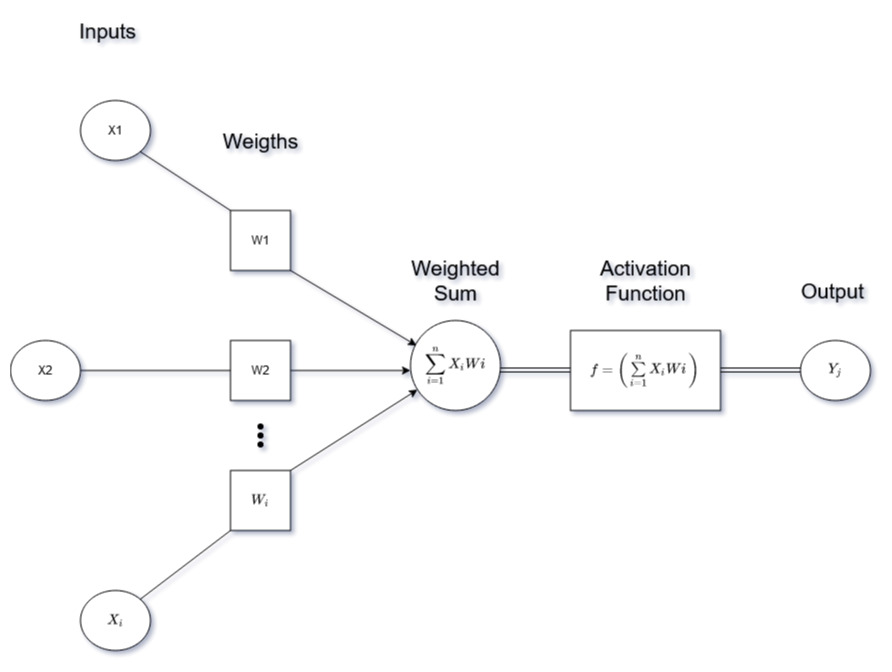
\includegraphics[width=0.6\textwidth]{images/Neuron.jpg}
\caption{Artificial Neuron}
\centering
\label{fig:neuron}
\end{figure}


Figure \ref{fig:nn} is an example of a feedforward multilayer neural network, also known as multilayer perceptron, where every node is connected to the next layer besides the output nodes, that can or can not be connected depending on the architecture of the neural network. 


\begin{figure}[H]
\centering
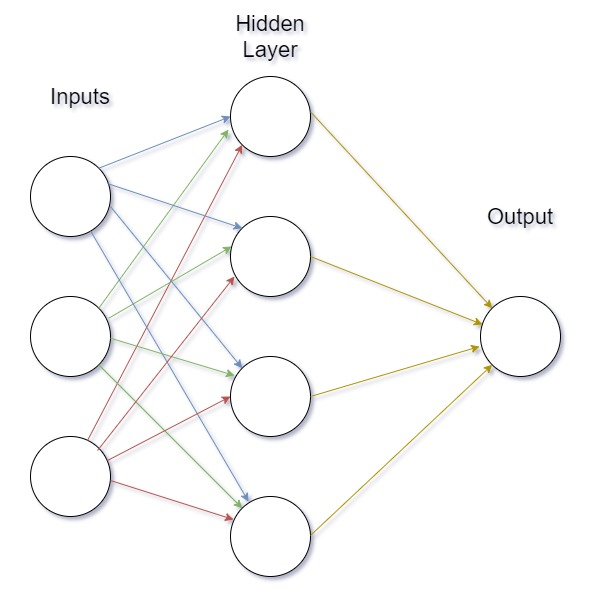
\includegraphics[width=0.5\textwidth]{images/nn.jpg}
\caption{Feedforward Multilayer Neural Network}
\centering
\label{fig:nn}
\end{figure}



\subsection{Activation Functions}



%Neural Netowkrs

\clearpage{\thispagestyle{empty}\cleardoublepage}
\section{Generative Adversarial Networks}

\subsection{\acs{GAN}}
The Generative Adversarial Network is an architecture that uses two neural networks: the generator and the discriminator, which compete against each other continuously, as if they were in a game. 


\par The function of the generator is, given a random noise, to generate new data instances that are synthetic, but need to be as real as possible so it can fool the discriminator. The generative models tend to model the distribution between classes, which means, that it tries to find the right data to reach a certain goal. The generator adapts its next generation according to if it has or has not succeeded on fooling the discriminator.


\par On the other hand, the discriminator evaluates the image that was generated. The discrimination models learn the correlation between the data and the corresponding output, classifying future data using that correlation. 



\par As we can see in figure \ref{fig:gan}, the generator takes random points from the latent space as input and from those points it generates an image. The latent space is usually 100-dimensional array with each element being a random value from the Gaussian Distribution figure \ref{fig:gauss} with a mean of zero. The discriminator is then going to receive this image as input along with real images from the dataset, and has to learn which ones are the fake images and which are the real ones.



\begin{figure}[H]
\centering
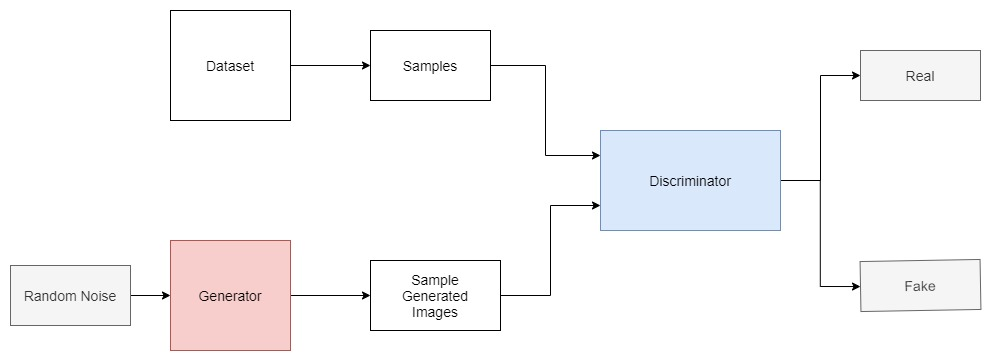
\includegraphics[width=1\textwidth]{images/GAN.jpg}
\caption{Generative Adversarial Network Architecture}
\centering
\label{fig:gan}
\end{figure}



\begin{figure}[H]
\centering
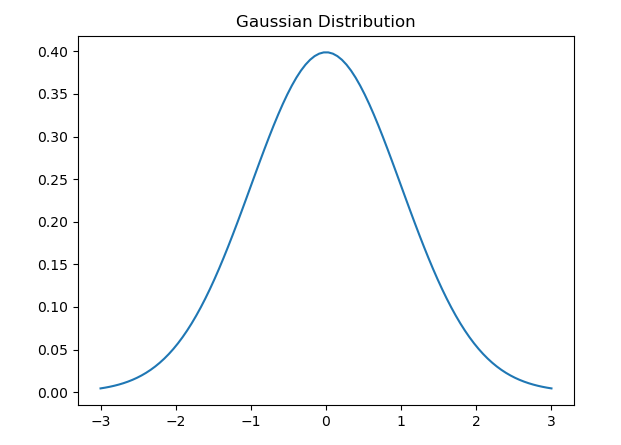
\includegraphics[width=0.8\textwidth]{images/GaussianDistribution.png}
\caption{Gaussian Distribution}
\centering
\label{fig:gauss}
\end{figure}


\subsection{Conditional GANs}

As an extension of the Generative Adversarial Networks there are the \textbf{Conditional Generative Adversarial Networks}. 

\par These models are used when the discriminator and the generator need to be conditioned on some additional information, usually, a class. The condition is passed as an additional input layer and then concatenated with the input image.



\begin{figure}[!thb]
\centering
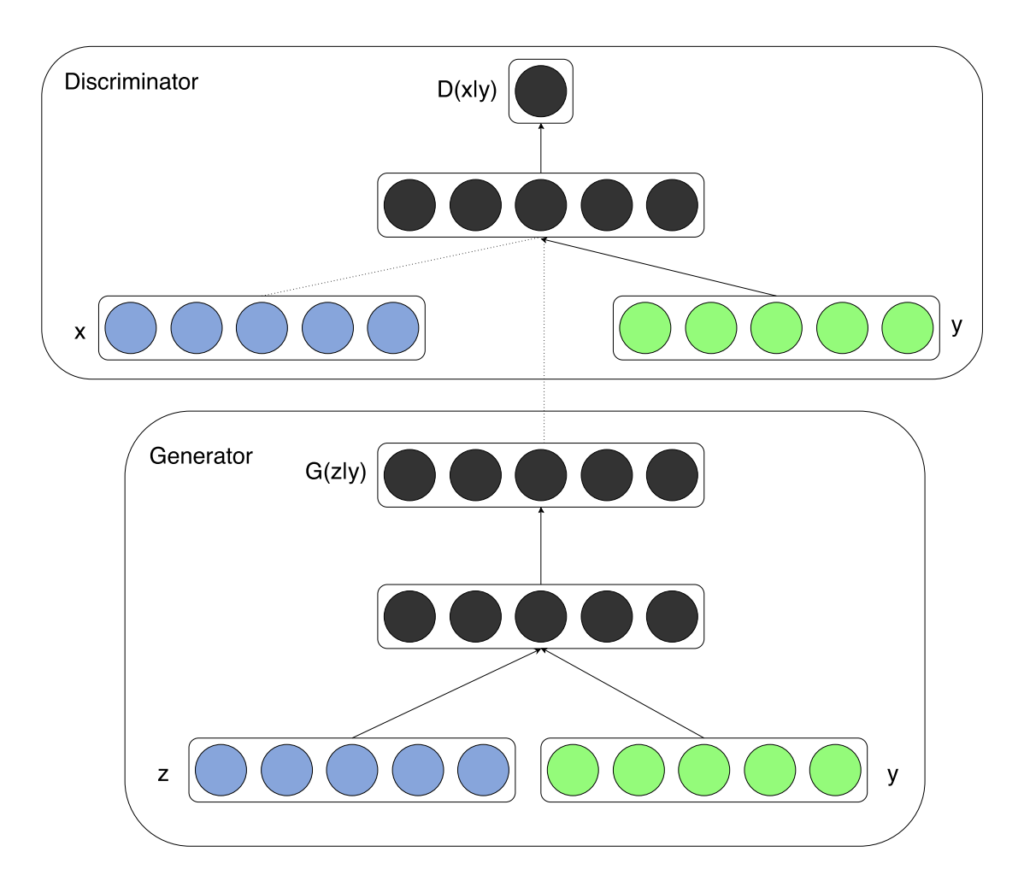
\includegraphics[width=300pt]{images/cGANs.png}
\caption{Conditional GAN architecture}
\centering
\end{figure}



In this architecture  we can see that in the Conditional Generative Adversarial Networks, both the discriminator and the generator, instead of only having the normal input, the \textbf{x}, they now also receive a condition, the \textbf{y}. The condition is then encoded, reshaped and concatenated with the input image.




\clearpage{\thispagestyle{empty}\cleardoublepage}


\chapter{Proposed Methods}
\label{chap:cganimp}

\section{\ac{CGAN}}
    \subsection{Setup}
    \label{sec:cgansetup} 
    \begin{itemize}
            \item \textbf{Language}: Python;
            \item \textbf{\acs{IDE}}: PyCharm; 
            \item \textbf{Framework}: Keras;
            \item \textbf{Model Visualization}: Netron.
    \end{itemize}


    
    \subsection{Dataset}
    \label{sec:cgandata}
    
    The dataset used for this project is split into 9 different folders, where each folder represents a different characteristic and inside contains all the respective images. 
    
    \par
    
    The 9 different characteristics are: eyebrow distribution, eyebrow size, eyebrow shape, eyelashes size, eyelids shape, iris color, skin color, skin texture and spots. In order to better analyse the dataset content I will describe how the characteristics are distributed in it and further into the report this is going to help us draw conclusions on why some problems occur.
    
    
    \begin{table}
    \begin{center}
    \begin{tabular}{ |c|c|c|c| } 
    \hline
    Eyebrow Distribution & Occurrences & Relative Frequency \\
    \hline
         0 - Sparse &  1679 & 16\% \\ 
        1 - Average & 5300 & 52\% \\ 
        2 - Dense & 3271  & 32\% \\ 
    \hline
    \end{tabular}
    \caption{Eyebrow distribution occurrences in the dataset.}
    \label{tab:edrist}
    \end{center}
    \end{table}
    
    
    \begin{table}
    \begin{center}
    \begin{tabular}{ |c|c|c|c| } 
    \hline
    Eyebrow Shape & Occurrences & Relative Frequency \\
    \hline
        0 - Angular &  1737 & 17\% \\ 
        1 - Straight & 3996 & 39\% \\ 
        2 - Round & 4431 & 43\% \\ 
        3 - S Shape & 86 & 1\% \\ 

    \hline
    \end{tabular}
    \caption{Eyebrow shape occurrences in the dataset.}
    \label{tab:eshape}
    \end{center}
    \end{table}
    
    
        
    \begin{table}
    \begin{center}
    \begin{tabular}{ |c|c|c|c| } 
    \hline
    Eyebrow Size & Occurrences & Relative Frequency\\
    \hline
        0 - Small &  1954 & 19\% \\ 
        1 - Medium & 4029 & 39\% \\ 
        2 - Large & 4267 & 42\% \\ 

    \hline
    \end{tabular}
    \caption{Eyebrow size occurrences in the dataset.}
    \label{tab:esize}
    \end{center}
    \end{table}
    
    
    
    
       \begin{table}
    \begin{center}
    \begin{tabular}{ |c|c|c|c| } 
    \hline
    Eyelashes Size & Occurrences & Relative Frequency\\
    \hline
        0 - Small & 3060 & 30\% \\ 
        1 - Medium & 5212 & 51\% \\ 
        2 - Large & 1978 & 19\% \\ 

    \hline
    \end{tabular}
    \caption{Eyelashes size occurrences in the dataset.}
    \label{tab:elashessize}
    \end{center}
    \end{table}
    
    
    \begin{table}
    \begin{center}
    \begin{tabular}{ |c|c|c|c| } 
    \hline
    Eyelids Shape & Occurrences & Relative Frequency\\
    \hline
        0 - Normal &  3915 & 38\% \\ 
        1 - Fall & 6335 & 62\% \\ 

    \hline
    \end{tabular}
    \caption{Eyelids shape occurrences in the dataset.}
    \label{tab:elidsshape}
    \end{center}
    \end{table}
    
    
     \begin{table}
    \begin{center}
    \begin{tabular}{ |c|c|c|c| } 
    \hline
    Iris Color & Occurrences & Relative Frequency\\
    \hline
        0 - Blue &  1448 & 14\% \\ 
        1 - Green & 698 & 7\% \\ 
        2 - Brown & 4171 & 41\% \\ 
        3 - Dark Brown & 3933 & 38\%\\ 


    \hline
    \end{tabular}
    \caption{Iris color occurrences in the dataset.}
    \label{tab:iriscolor}
    \end{center}
    \end{table}
    
    
    
      \begin{table}
    \begin{center}
    \begin{tabular}{ |c|c|c|c| } 
    \hline
    Skin Color & Occurrences & Relative Frequency\\
    \hline
        0 - Black &  180 & 2\% \\ 
        1 - Tanned & 333 & 3\% \\ 
        2 - White & 8836 & 86\% \\ 
        3 - Extreme White & 901 & 9\% \\ 


    \hline
    \end{tabular}
    \caption{Skin color occurrences in the dataset.}
    \label{tab:skincolor}
    \end{center}
    \end{table}
    
    
        
      \begin{table}
    \begin{center}
    \begin{tabular}{ |c|c|c|c| } 
    \hline
    Skin Texture & Occurrences & Relative Frequency\\
    \hline
        0 - Young &  1949 & 19\% \\ 
        1 - Young Plus & 6470 & 63\% \\ 
        2 - Adult & 1231 & 12\% \\ 
        3 - Aged & 600 & 6\% \\ 


    \hline
    \end{tabular}
    \caption{Skin texture occurrences in the dataset.}
    \label{tab:skin_text}
    \end{center}
    \end{table}
    
    
           
      \begin{table}
    \begin{center}
    \begin{tabular}{ |c|c|c|c| } 
    \hline
    Spots & Occurrences & Relative Frequency\\
    \hline
        0 - No Spots &  8184 & 80\% \\ 
        1 - 1 Spot & 630& 6\% \\ 
        2 - 2 Spots & 1436 & 14\% \\ 


    \hline
    \end{tabular}
    \caption{Spots occurrences in the dataset.}
    \label{tab:spots}
    \end{center}
    \end{table}
    
    
    
    \subsection{Generator model}
    \label{sec:cgangen}
    
    \begin{figure}[H]
    \centering
    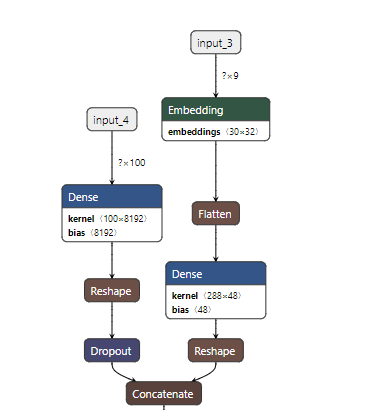
\includegraphics[width=0.5\textwidth]{images/generator_1.png}
    \caption{Generator input layers.}
    \centering
    \label{fig:neuron}
    \end{figure}
    
    
      
    \begin{figure}[H]
    \centering
    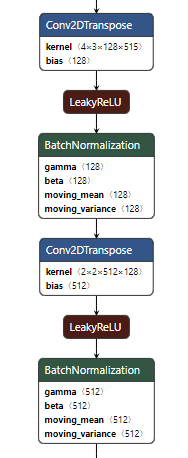
\includegraphics[width=0.25\textwidth]{images/generator_2.png}
    \caption{Generator upsample layers.}
    \centering
    \label{fig:neuron}
    \end{figure}
    
    
      
    \begin{figure}[H]
    \centering
    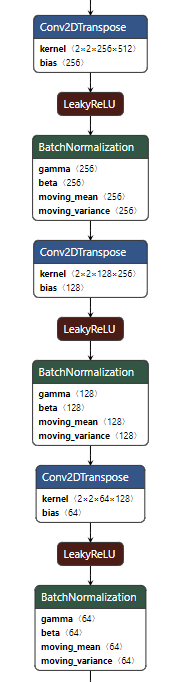
\includegraphics[width=0.25\textwidth]{images/generator_3.png}
    \caption{Generator upsample layers.}
    \centering
    \label{fig:neuron}
    \end{figure}
    
    
    
      
    \begin{figure}[H]
    \centering
    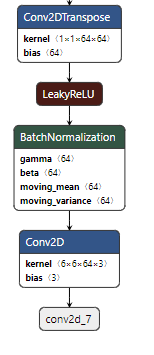
\includegraphics[width=0.25\textwidth]{images/generator_4.png}
    \caption{Generator complexity and output layers}
    \centering
    \label{fig:neuron}
    \end{figure}
    
    
    
    \subsection{Discriminator model}
    \label{sec:cgandiscri}
    
    
    
    
    \begin{figure}[H]
    \centering
    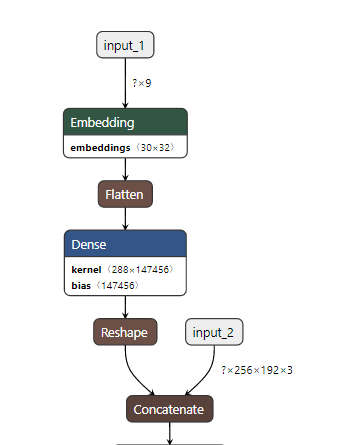
\includegraphics[width=0.45\textwidth]{images/discriminator_1.png}
    \caption{Discriminator input layers.}
    \centering
    \label{fig:disc}
    \end{figure}
    
    
        
    \begin{figure}[H]
    \centering
    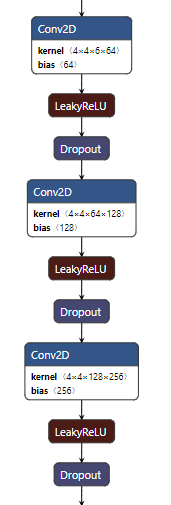
\includegraphics[width=0.2\textwidth]{images/discriminator_2.png}
    \caption{Discriminator downsample layers.}
    \centering
    \label{fig:disc}
    \end{figure}
    
    
    
        
    \begin{figure}[H]
    \centering
    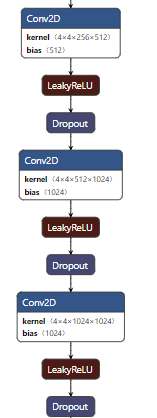
\includegraphics[width=0.2\textwidth]{images/discriminator_3.png}
    \caption{Discriminator complexity layers.}
    \centering
    \label{fig:disc}
    \end{figure}
    
    
    
        
    \begin{figure}[H]
    \centering
    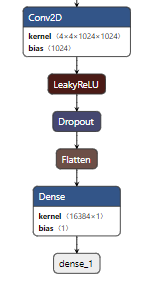
\includegraphics[width=0.2\textwidth]{images/discriminator_4.png}
    \caption{Discriminator output layer.}
    \centering
    \label{fig:disc}
    \end{figure}
    

\section{Search algorithms}
Due to the fact that with the current 9 characteristics there are 41472 possible combinations for an image, I had to implement various algorithms that would efficiently search the best fitting combination for a given image. This section explains the implementation of these algorithms along with the advantages and disadvantages of each one. 
\label{sec:search}


\subsection{Setup}
\label{sec:search_setup}
\begin{itemize}
    \item \textbf{Language}: Python;
    \item \textbf{\acs{IDE}}: PyCharm.
\end{itemize}

\subsection{Brute Force}
\label{sec:cganbrute}
The brute force algorithm is the most basic and easier algorithm implemented. It consists on a script that iterates through all the possible combinations and saves each combination and its respective probability in a list. After iterating through all combinations, the script outputs the combination with the highest probability.   
    \subsubsection{Advantages and Disadvantages}
    Since the algorithm needs to iterate through all the possible combinations, it is not efficient. In subsection \ref{sub:brute} we analyse further the efficiency of this algorithm, also, with this algorithm we always get the combination with the highest probability which can be a problem given that the discriminator's model is not perfect.
    \label{sec:bruteadv}

\subsection{Safe Lock}
\label{sec:lock}
Professional robbers break into some safes through the sound of the pins, whenever they unlock a pin and it makes a click and it means that the combination they are inserting is correct. Inspired by this idea, I decided to implement a similar algorithm to this system, the safe lock algorithm.

\par

We can compare the safe bins to the characteristics of a combination, and we will keep changing a random characteristic until we hear the "click", which in our case, is when the probability increases. By using this method we can keep changing characteristics one by one until we reach a certain number of tries that have not increased the probability, meaning that we already have the combination with the highest probability.



    \subsubsection{Advantages and Disadvantages}
    \label{sec:safeadv}
    When compared to the brute force algorithm, this one is a huge improvement when it comes to  efficiency, in subsection \ref{sub:safe} we will further analyse these efficiency improvements.
    
    \par
    
    However, this algorithm shares the same problem with the brute force method, this is, they always output the combination with the highest probability. In subsection \ref{ssec:highm} we will be able to identify this problem and why it is not always good to search for the combination with the highest probability.
    


\subsection{A* Algorithm}
\label{sec:star}
The A* algorithm is one of the best techniques used in path-finding and graph traversals \cite{A*}. The core of this algorithm is on the heuristics, based on these, it will find the best path to a given destination. Usually, the A* has 2 heuristics: the first heuristic returns the movement cost from the starting point to a given node, the other heuristic returns the estimated movement cost from the current node to the final destination.

\par

In this project we are not dealing with graphs and neither with fixed destinations, and because of this, the algorithm implemented in this system differs from the original A* implementation. 

\par
In this system the two heuristics implemented are the following: one heuristic that returns the difference between the probability of the current combination and the probability of a given successor, and the other one returns the estimated probability remaining from the current combination to the average probability, which corresponds to the final destination. Since we can not assign a fixed combination as the destination, we set a probability to do this job. This probability is not random, we start by doing research on what are the probabilities outputted by the discriminator to the real combinations of images. After doing the average of these outputs, we obtain the average probability of the actual combinations of the images, and we can set it as a destination for the A* algorithm.


    \subsubsection{Advantages and Disadvantages}
    One of the biggest advantages of this algorithm is the fact that it takes in consideration the discriminator's mistakes. In subsection \ref{astaralg} we will further analyse why this is such an important factor to take into account when searching for the best fitting combination.
    \par
    
    The major disadvantage in this algorithm is the fact that it does not have a fixed time to execute. Since it starts with a random combination and has to find its way to the destination, it all depends on the starting combination probability, for instance, if it is close to the probability set as destination then the algorithm will execute in no time, or, if the start probability is really far from the destination, it will take more time. 
    
    \par
    In conclusion, the A* algorithm loses some efficiency when compared to the safe lock algorithm but it is has more chances of outputting the correct combination for a given image.
    
    \label{sec:staradv}


\section{Classification Algorithms Implementation}
\label{chap:decisionalg}
The last part of the system has to be able to receive two combinations and classify them as part of the same person or not. Developing a model that can output this classification is essential due to the fact that the A* algorithm does not always output the same combination for a given image. For instance, if we have two images from the same person, there is a chance that the combination outputted is different for each image, and we have to take that in consideration and find patterns between these different combinations in order to analyse what characteristics are different and which ones are usually the same for the two images.  

\par

In order to develop a model that would find these patterns and classify two combinations I implemented two classification models: a simple multilayer perceptron and the c4.5 algorithm used to generate a decision tree, developed by Ross Quinlan. 

\par

This section explains all the methods used in the implementation of these two algorithms.

\subsection{Dataset}
Figure \ref{fig:class} shows a sample of the training dataset. The complete dataset consists in 30750 records, 24000 for training and 6750 for test, and each record has two combinations and the respective label. For each image it was generated a single correct record and two false records. 



\begin{figure}[H]
\centering
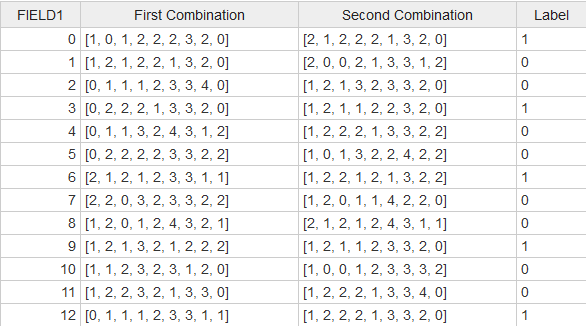
\includegraphics[width=0.7\textwidth]{images/dataset.png}
\caption{Training dataset sample.}
\centering
\label{fig:class}
\end{figure}



\subsection{\ac{MLP}}
\label{sec:mlp} 
Figure \ref{fig:mlparch} represents the implemented multilayer perceptron's architecture. Primarily we define the two inputs with the size of 9. We pass each input through an embedding layer, this is going to map the 9 different characteristics from the input combination to a different 32 element vector representation that will be learned by the discriminator. The outputs from these layers will be flattened into a dense layer with 128 nodes with no activation function, and concatenated to a dense layer with 256 nodes. After the concatenation of the inputs, we define one more hidden dense layer with 128 nodes with ReLu as the activation function. Finally, we define the output layer with sigmoid as the activation function.

\par





\begin{figure}[H]
\centering
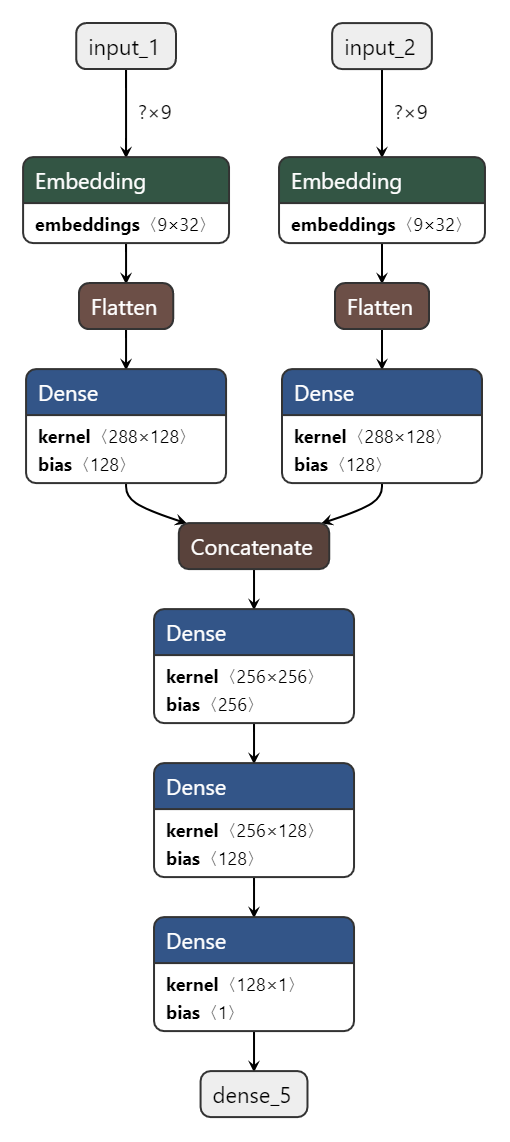
\includegraphics[width=0.4\textwidth]{images/mlp_model.png}
\caption{\acs{MLP} architecture.}
\centering
\label{fig:mlparch}
\end{figure}



\subsection{C4.5 Algorithm}
\label{sec:alg45}
Since the core of this project is the interpretability of the system, makes sense to implement a decision tree classifier, since these can explain with a lot more detail why they made a decision and what was taken in consideration.

\par

The C4.5 algorithm generates a decision tree from training data using the concept of information entropy \cite{entropy}, this decision tree can then be used for classification. In order to understand how the algorithm generates a decision tree we have to take into account 3 base cases of the algorithm:
\begin{itemize}
    \item All the samples from the training dataset belong to the same class, in this case it returns a leaf to the decision tree that predicts that class.
    \item Features do not provide any information gain, in this case it returns a leaf to the decision tree that predicts the most frequent class.
    \item Class was not yet observed, in this case it also returns a leaf to the decision tree that predicts the most frequent class.
\end{itemize}


The algorithm starts by checking if any of the cases mentioned above occur. After that, it splits 

\begin{equation}   
    Entropy(D) = -\sum\limits_{i=0}^{n}p(x)\log_2 p(x)
    \label{eq:entropy}
\end{equation}






\clearpage{\thispagestyle{empty}\cleardoublepage}

\chapter{Experiments and Discussions}


\section{\acs{CGAN} Experiments}
In this section, I will explain the various attempts at implementing the \acs{CGAN}, the parameters that I have tried to adjust and my opinion on why some worked and some did not.


\subsection{Mode Collapse}
One of the problems that is very common in \acs{GAN}s is the mode collapse situation that occurs on the generator at the training phase. After a certain epoch, the generator will start to produce an insignificant diversity of samples in order to fool the discriminator and will not improve for the rest of the training phase.

\par

The reason behind this is simple, but extremely hard to solve: if we take as an example the dataset used for this project and the characteristics of each image, the training of the model will be something like this. The generator will find out that the discriminator is being fooled by images that have blue eyes, therefore, it will produce more images with blue eyes. However, the discriminator also learns that the generator is trying to produce more images with blue eyes in order to make them look real, so, it starts to adapt to this changes. This will lead to the generator having to find another way to fool the discriminator by producing samples of another eye color or characteristic with no variety whatsoever.

\par

Figure \ref{fig:mdcolap} shows some results I got on my first attempt at training the \acs{CGAN}. As we can see, mode collapse is clearly happening since there is no variety on the images generated. After some research, I tried changing the learning rates of both the discriminator and the generator to see if it made any difference and it happened to solve the problem, but not completely. At the beginning I had the generator and discriminator with the same learning rate, 0.0002. Nevertheless, after increasing the discriminator to 0.0003 I was able to see some improvement on the variety of the images that were generated as we can see in figure \ref{fig:nocola}. The reason this does not solve the problem completely is due to the fact that, later on the training phase, the generator will start to collapse again to a certain type of image.





\begin{figure}[H]
\centering
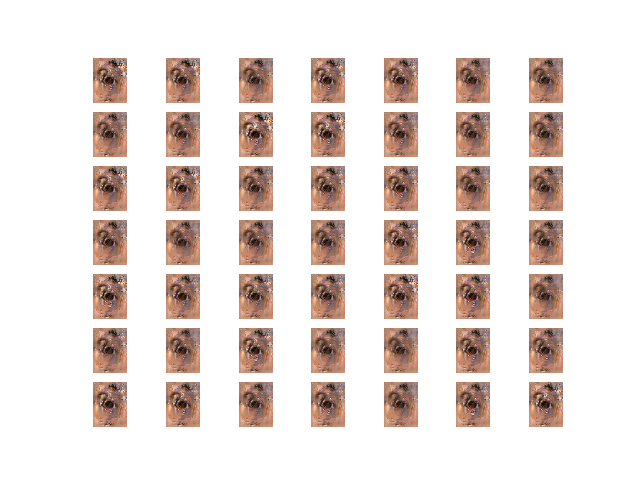
\includegraphics[width=1\textwidth]{images/mode_collapse.png}
\caption{Mode collapse, same learning rates.}
\centering
\label{fig:mdcolap}
\end{figure}





\begin{figure}[H]
\centering
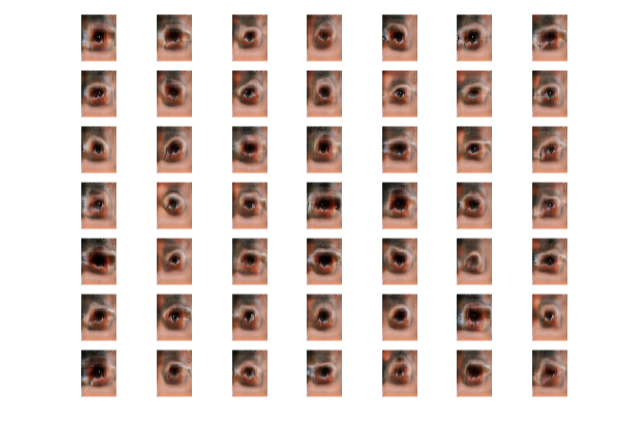
\includegraphics[width=1\textwidth]{images/No_collapse.png}
\caption{No mode collapse, different learning rates.}
\centering
\label{fig:nocola}
\end{figure}
 

\subsubsection{Discussion}
The mode collapse problem is something that I spent a great amount of time thinking about and trying to solve. After trying many values for the learning rate of both the discriminator and the generator, I can say that, even though it allows to play around with these values and get small improvements, it is not a complete solution to the problem. 


\par 

By adjusting the learning rates we are telling the model how quickly it should adapt to a certain problem, and by having the same values for both, it should mean that there is a balance between them and, since one learns along with the other, what ends up happening is that the generator enters this cycle of trying to fool the discriminator based on a low variety of characteristics and produces a small variety of images. Slightly increasing the learning rate of the discriminator helps to prevent the mode collapse because, that way, we give the discriminator a small starting advantage, therefore, it will be able to learn faster to distinguish the real images from the fake ones. That is why, the generator has to keep up by trying to generate a wider variety of images in order to be able to fool the discriminator.


\par

Even though, as I said before, adjusting the learning rates helps to get improvements, the major contributor to this problem, from my perspective and from all the experiments I have done, is the small variety of the images in the dataset.  INCLUIR REFERENCIA AOS DADOS DA DATASET COM DADOS QUE SUPORTAM A AFIRMAÇÃO- TODO





\subsection{Discriminator and Generator Complexity Balance}

Something that is really important when training a \acs{GAN} is the balance between the complexity of the discriminator and generator models, as this prevents one from having an advantage over the other one. On my first attempts, the discriminator model was much more complex than the generator-- this could be quickly figured out by analysing its output. Figure \ref{fig:morecomp} shows some of the generated images when the discriminator was more complex. This difference in complexity makes it so that the generator has no chance against the discriminator, and because of that, there is no improvement on the output images.



\begin{figure}[H]
\centering
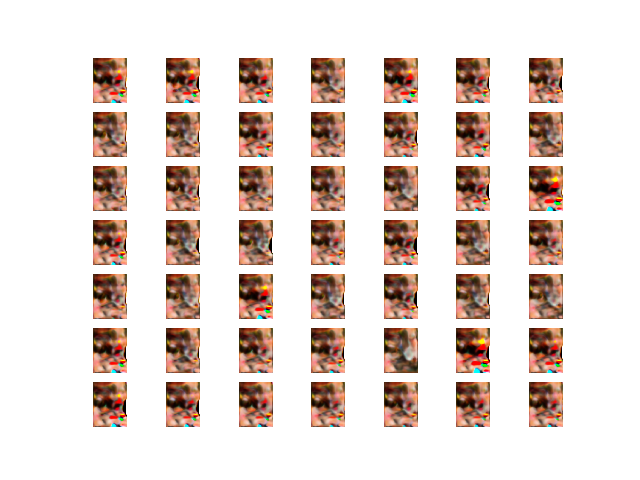
\includegraphics[width=1\textwidth]{images/more_complex.png}
\caption{Samples from the training phase where the discriminator has a higher complexity than the generator.}
\centering
\label{fig:morecomp}
\end{figure}
 


Instead of downgrading the discriminator's complexity, I upgraded the complexity of the generator by adding more layers, since this makes it easier for the model to recognize certain aspects of the input data. After this change, I was able to see some improvement on the images that were generated as shown in figure \ref{fig:samecomp}.



\begin{figure}[H]
\centering
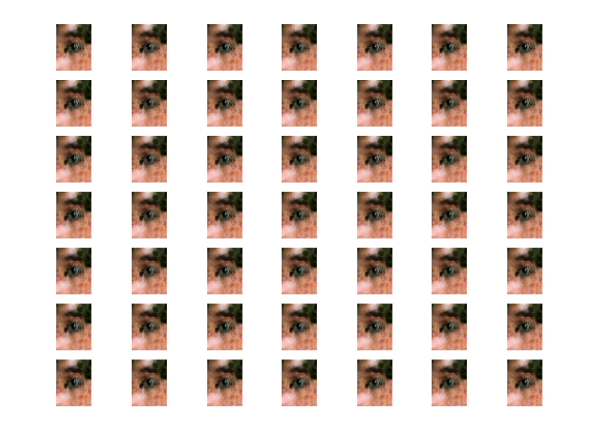
\includegraphics[width=1\textwidth]{images/same_complex.png}
\caption{Samples from the training phase where the discriminator has the same complexity than the generator.}
\centering
\label{fig:samecomp}
\end{figure}
 


\subsubsection{Discussion}
The challenge with increasing the generator's complexity is that it had to be perfectly tuned so that the same does not happen with the discriminator. And in my opinion, this was the most interesting part: trying to add layers to the model without overpowering it and in a way that it would be able to recognize more aspects of the input data, so, for instance, instead of taking into consideration onky the skin color of a certain image, it takes into consideration all the 9 characteristics.




\subsection{Upsampling2D Layer vs Conv2DTranspose}

As part of the generator model we have the layers that will upsample an image. As we can see in the section //TODO-> Implementação da GAN, generator model//, the used layer to upsample an image was the UpSampling2D. This choice of implementation was not random, after starting to study methods on how to implement these layers, the UpSampling2D and the Conv2DTranspose, I decided to try them both and analyse the differences in order to help me make a decision on which one to use. At first, I tried using the Conv2DTranspose layers to upsample the images on the generator, as we can see in figure \ref{fig:conv} the results were not particularly bad but they were "glitchy" and not smooth.  



\begin{figure}[H]
\centering
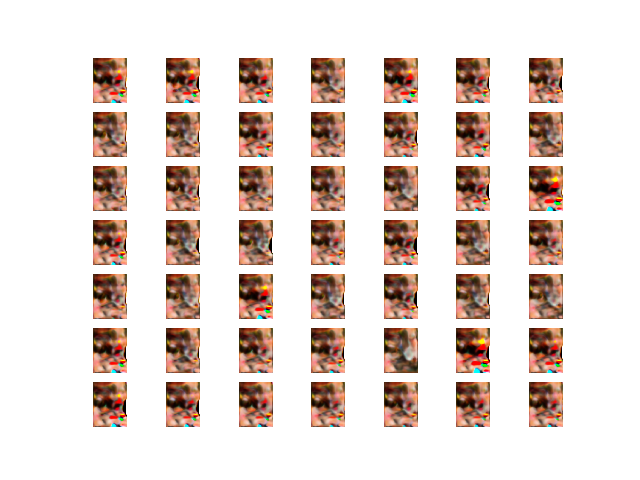
\includegraphics[width=1\textwidth]{images/conv.png}
\caption{Samples generated using Conv2DTranspose layers to upsample images.}
\centering
\label{fig:conv}
\end{figure}


On the other hand, when using the UpSampling2D layers to upsample images, the results were much better in terms of image quality, as we can see in figure \ref{fig:upsamp}, the upsampled images looked more natural and smoother.



\begin{figure}[H]
\centering
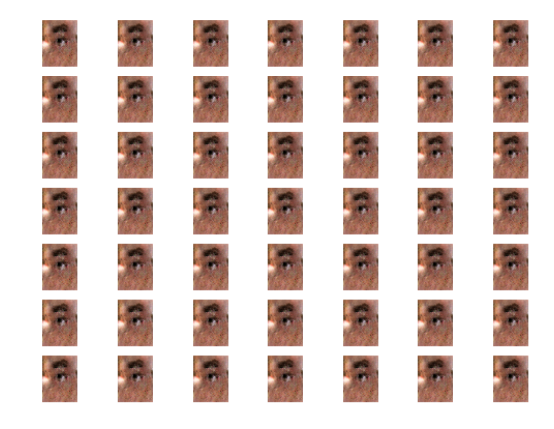
\includegraphics[width=0.9\textwidth]{images/upsample.png}
\caption{Samples generated using UpSample2D layers to upsample images.}
\centering
\label{fig:upsamp}
\end{figure}


\subsubsection{Discussion}
The need for transposed convolutions generally arises from the desire to use a transformation going in the opposite direction of a normal convolution \cite{2016arXiv160307285D}. 

\par

In this case we have the random noise and the characteristics as the generator's input, and we want to transform these inputs in an image. The results from the experiments came to confirm that using the Conv2DTranspose layers would be a better choice overall. This is due to the fact that while the UpSample2D layer only doubles each row and column of the matrix illustrated in figure \ref{fig:upsamp1}, the Conv2DTranspose is like an inverse convolutional layer, and because of this, instead of only doubling the row and column values, it receives as one of the inputs, the stride, which refers to the manner in which outputs in the feature map are laid down \cite{upsample}.

\par

In figure \ref{fig:upsamp2}, we can see that the output of the Conv2DTranspose layer is different because instead of just doubling the values of each column and row, it uses it's weights to learn how to upsample the image naturally and with more detail, although, in this example the weights are forced to be the same so we get an easier understanding on how it works.





\begin{figure}[H]
\centering
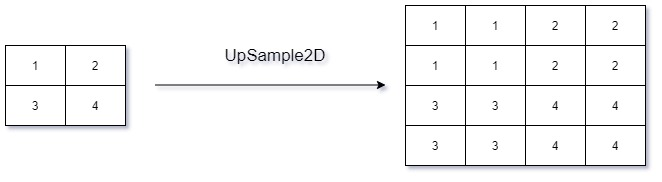
\includegraphics[width=0.9\textwidth]{images/sample1.jpg}
\caption{Example of an output of the UpSample2D layer.}
\centering
\label{fig:upsamp1}
\end{figure}



\begin{figure}[H]
\centering
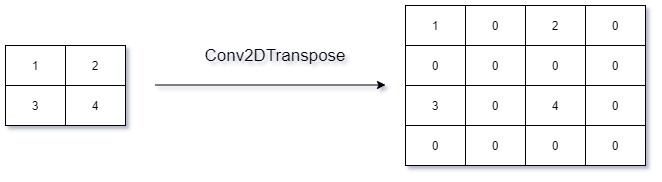
\includegraphics[width=0.9\textwidth]{images/upsample2.png}
\caption{Example of an output of the Conv2DTranspose layer.}
\centering
\label{fig:upsamp2}
\end{figure}



\subsection{LeakyReLU vs ReLU}


\subsubsection{Discussion}


\subsection{Adam Optimizer vs RMSProp Optimizer}

\subsubsection{Discussion}




\section{Search Algorithms Experiments}
In this section I am going to show and discuss the results of the search algorithms implemented in this project.

\subsection{Brute Force}
\label{sub:brute}
By using the brute force algorithm the estimated time to find the best combination of characteristics is 2 minutes. Even though this is the most accurate method, meaning that it will always find the highest probability combination that matches a certain image, it is not efficient whatsoever.


\par

One of the reasons this would be a bad choice is the fact that maybe later in future work, more characteristics will be added and the number of possible combinations will increase exponentially, and with it, the running time of the algorithm. 

Another reason on why it is not the best method, is the simple fact that, the discriminator model is not completely accurate, meaning that, even if it gives a certain combination of characteristics a very high probability, it does not necessarily mean that it is the correct one for the image.


\subsubsection{Discussion}
Thinking about this algorithm only makes sense if we don't have another alternative for testing results or if we are working with a relative small amount of possible combinations. At first I was thinking about discarding this algorithm due to the fact that the SOCIALAB's computer was training another model, and since I was having problems setting up my GPU to run these models, I tried running it on my computer's \acs{CPU} and the estimated time to run this algorithm for one image was 4 hours.

\par

These previously mentioned problems motivated me into implementing more efficient algorithms and that can adapt to any future extensions that may come this project.


\subsection{Safe lock}
\label{sub:safe}
By using the safe lock algorithm, explained in the (section 3.2.1 //TODO ref), I got much better results. The estimated time to find the best combination possible for an image with this algorithm is 8 seconds, which compared to the brute force, is a huge improvement on efficiency. 


\subsubsection{Discussion}
In my opinion and as the results show, this algorithm is a huge improvement when comparing it to the brute force one, but they both suffer from the same problem. The fact that the correct combination for a certain image is always the one with the higher probability, leads to mistakes in these algorithms. In \autoref{ssec:highm} we will be able to analyse further this problem.


\subsection{Safe Lock and Brute Force Confusion Matrices}
\label{ssec:highm}
 Figure \ref{fig:confexam} illustrates a confusion matrix, also known as an error matrix, which is able to analyse the performance of the predictive model and give detailed information about what classes are useful to the model and which ones are creating problems.
 


\begin{figure}[H]
\centering
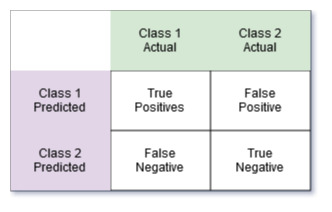
\includegraphics[width=0.65\textwidth]{images/confusion_example.jpg}
\caption{Confusion matrix example.}
\centering
\label{fig:confexam}
\end{figure}



With the purpose of analysing further the discriminator model, I decided to generate confusion matrices for all the characteristics predicted by the safe lock algorithm and comparing them with the actual image characteristics. 

\par

In the following matrices the values are normalized by columns for an easier interpretation and the overall accuracy was calculated by dividing the number of entries in the diagonal by the total number of entries in the matrix.


\subsubsection{Eyebrow Distribution}

Figure \ref{fig:eyebrow_lock_distribution} displays the confusion matrix of the eyebrow distribution characteristic. By analysing the matrix we notice that most of the times the discriminator predicts an average distribution. In 61\% of the images where the actual characteristic is average, the model also predicts it as average, however, in 26\% of these images it confuses them with dense distribution.


\par

Furthermore, the model tends to predict average in spite of the fact that it is not the actual class. For instance, in 57\% of the images where the actual class was sparse, the model predicted average. This is also noticeable in cases where the actual class of the image is dense, and the model predicts average in 53\% of the images.    


\par

Having this tendency to confuse dense distribution and sparse distribution with average distribution leads to the accuracy of the model, regarding this characteristic, to be 48\%. 

\begin{figure}[H]
\centering
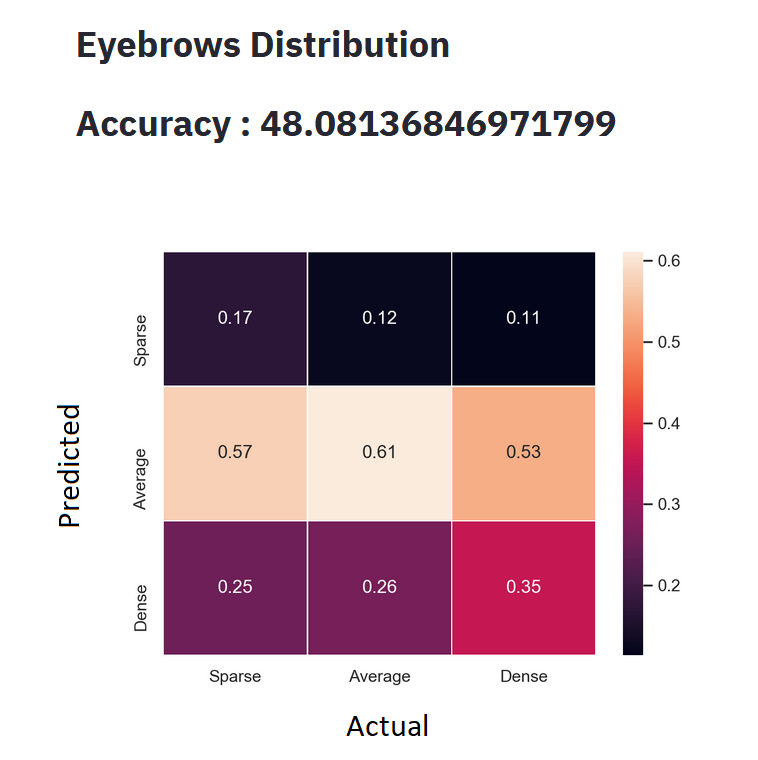
\includegraphics[width=0.65\textwidth]{images/eyebrows_lock_distribution.png}
\caption{Eyebrow distribution confusion matrix.}
\centering
\label{fig:eyebrow_lock_distribution}
\end{figure}



\subsubsection{Eyebrow Shape}
Figure \ref{fig:eybrows_lock_shape} displays the confusion matrix of the eyebrow shape characteristic. In this matrix we notice that whenever an image has an actual Sshape eyebrow, the model rarely predicts it correctly. In table \ref{tab:eshape} we can see that the amount of samples of Sshape is extremely low compared to the others, and thus, leading to the bad accuracy in terms of this class.

\par

When it comes to other classes the model tends to predict the round shape correctly 49\% of the times, for straight shape it has an accuracy of 36\% and for angular shape it has an accuracy of 20\%. Since the values of the matrix are distributed all around the matrix, this means that there is an high level of confusion by the model when it comes to this characteristic.

\begin{figure}[H]
\centering
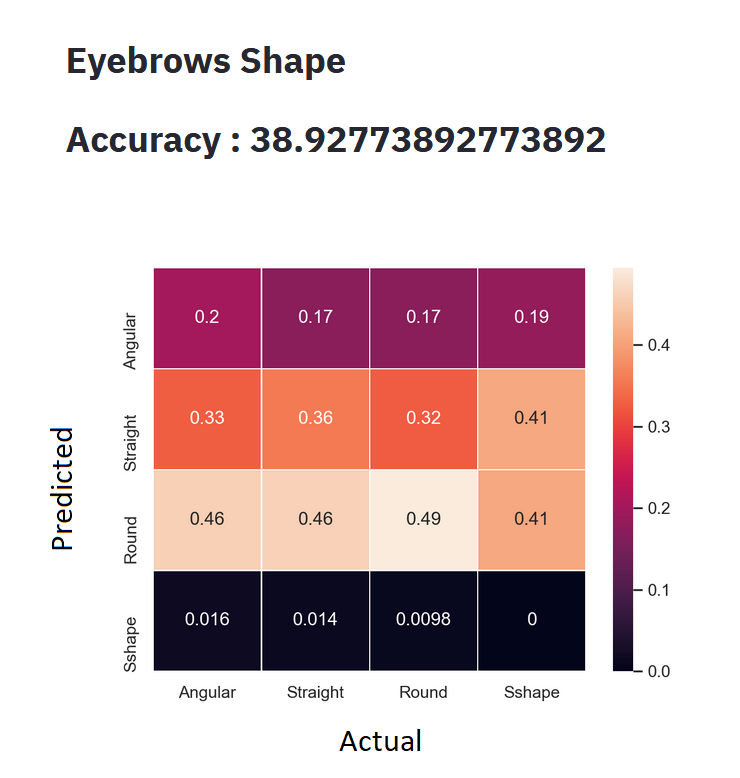
\includegraphics[width=0.65\textwidth]{images/eyebrows_lock_shape.png}
\caption{Eyebrow shape confusion matrix.}
\centering
\label{fig:eybrows_lock_shape}
\end{figure}





\subsubsection{Eyebrow Size}
Figure \ref{fig:eyebrow_lock_size} displays the confusion matrix of the eyebrow size characteristic. What stands out in this confusion matrix is that there are a great quantity of dispersed values all over the matrix, which means that the discriminator tends to often confuse classes when it comes to this specific characteristic and that is noticeable by the overall accuracy of 38,5\%.

\par

 In this matrix we notice that the discriminator almost never predicts small size. Consequently, images where the actual size is small, the model only predicts it correctly 26\% of the times. When it comes to the other classes, in images where the actual size is medium the model correctly predicts it 44\% of those images and tends to confuse 37\% of them with large size. The same happens to the large size, when images have this size, the model only predicts it correctly 40\% and confuses it with the medium size 44\% of the times.    



\begin{figure}[H]
\centering
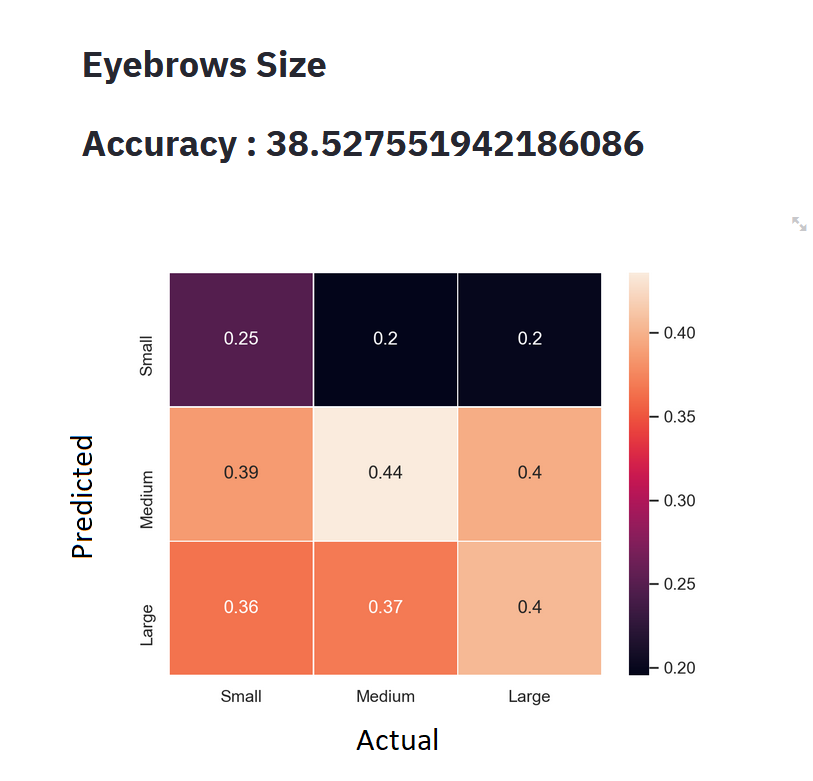
\includegraphics[width=0.65\textwidth]{images/eyebrows_lock_size.png}
\caption{Eyebrow size confusion matrix.}
\centering
\label{fig:eyebrow_lock_size}
\end{figure}


\subsubsection{Eyelashes Size}
Figure \ref{fig:eyelashes_lock_size} displays the confusion matrix of the eyelashes size characteristic. In this matrix we notice that the model tends to predict class 1 more than the rest of the classes, once again, this is due to the fact that the amount of samples in the dataset are not uniform and there are more samples of class 1 than the rest, as shown in table \ref{tab:elashessize}. When it comes to accuracy, the model predicts correctly 55\% of the times where the actual class is 1. Although, when predicting other images where the the actual class is 0 and class 2, the model tends to predict them as class 1 most of the times. 


\begin{figure}[H]
\centering
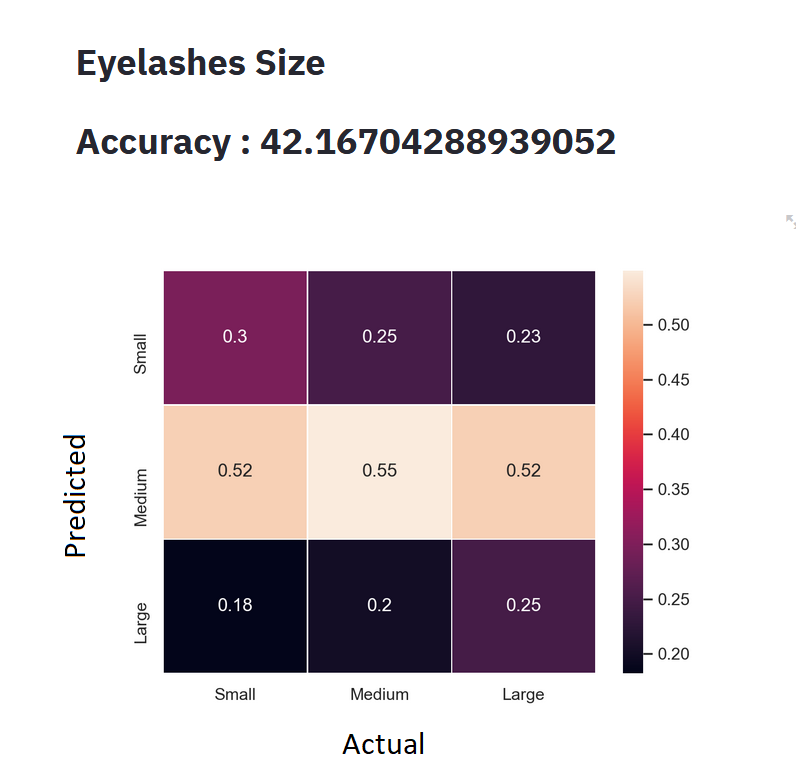
\includegraphics[width=0.65\textwidth]{images/eyelashes_lock_size.png}
\caption{Eyelashes size confusion matrix.}
\centering
\label{fig:eyelashes_lock_size}
\end{figure}


\subsubsection{Eyelids Shape}
Figure \ref{fig:eyelids_lock_shape} displays the confusion matrix of the eyelids shape characteristic.
Once again we notice the problem where the model tends to predict one class over the others, in this case, the discriminator predicts fall 67\% of the times where the actual shape is fall which is a good accuracy, but also predicts 62\% of the times fall when the actual shape is normal. This problem is also related the amount of samples in the dataset, as we can see in \ref{tab:elidsshape} the amount of samples of fall is significantly higher than the samples of normal shape.

\begin{figure}[H]
\centering
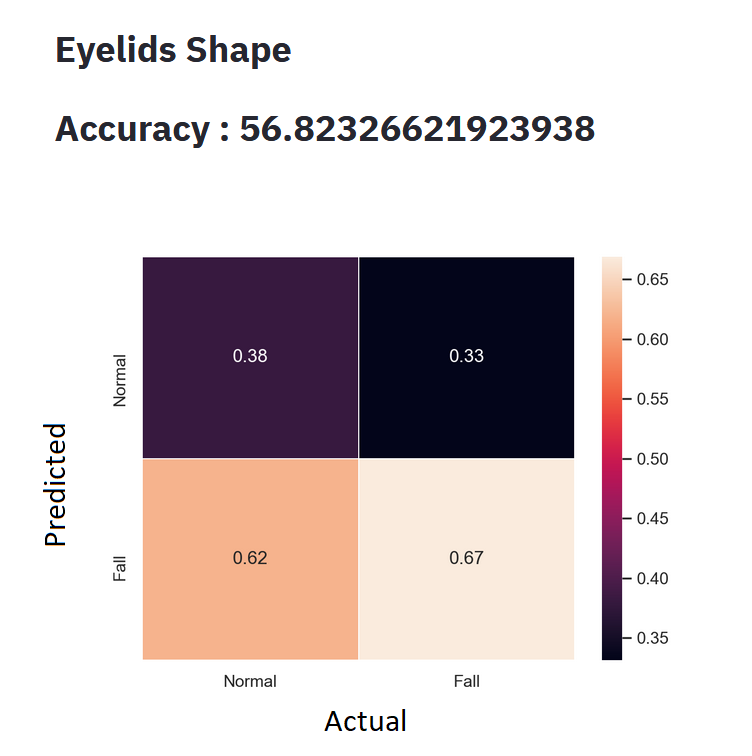
\includegraphics[width=0.65\textwidth]{images/eyelids_lock_shape.png}
\caption{Eyelids shape confusion matrix.}
\centering
\label{fig:eyelids_lock_shape}
\end{figure}


\subsubsection{Iris Color}
Figure \ref{fig:Iris_lock_color} displays the confusion matrix of the iris color characteristic. The iris color characteristic is one that the model has a very hard time identifying, this is due to the fact that there are not enough images in the dataset with blue eyes and green eyes that allow the model to learn how to recognize them, and this is why we see so many predictions of brown and dark brown eyes, and not that many with blue and green eyes.


\par

 By analysing the matrix we notice that the model tends to confuse the brown eyes with the dark brown eyes, this is understandable since even humans sometimes have difficulties to distinguish the two, but we see that 46\% of the times where the color was brown the model predicted it correctly even though in 28\% of the images it confused the brown eyes with the dark brown eyes. This scenario also happens the other way around, where the model predicts correctly 33\% of the times where the color is dark brown but confuses them with brown 41\% of the times. 
 
 \par
 
 These problems lead to the overall accuracy of the model towards this characteristic being low since most of the samples are of color brown and dark brown.

\begin{figure}[H]
\centering
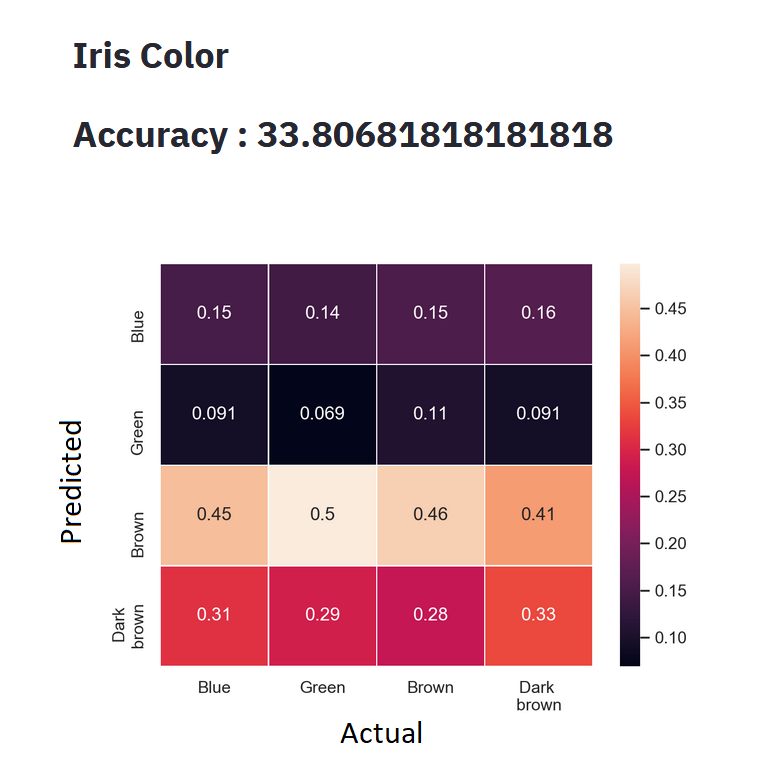
\includegraphics[width=0.65\textwidth]{images/Iris_lock_color.png}
\caption{Iris color confusion matrix.}
\centering
\label{fig:Iris_lock_color}
\end{figure}


\subsubsection{Skin Color}
Figure \ref{fig:skin_lock_color} displays the confusion matrix of the skin color characteristic. In this matrix we notice that white color is predominant over the other 3 colors, this is due to the amount of samples in the dataset of this class, as we can see in the table \ref{tab:skincolor}, white has around 8000 samples when the other classes have no more than a thousand samples each. 


\par

The reason for the overall accuracy being so high, is based on the fact that since the majority of images have white color, the model is going to predict correctly for these images. But when it tries to predict another class that is not white, it is not able to predict it correctly.
 
\begin{figure}[H]
\centering
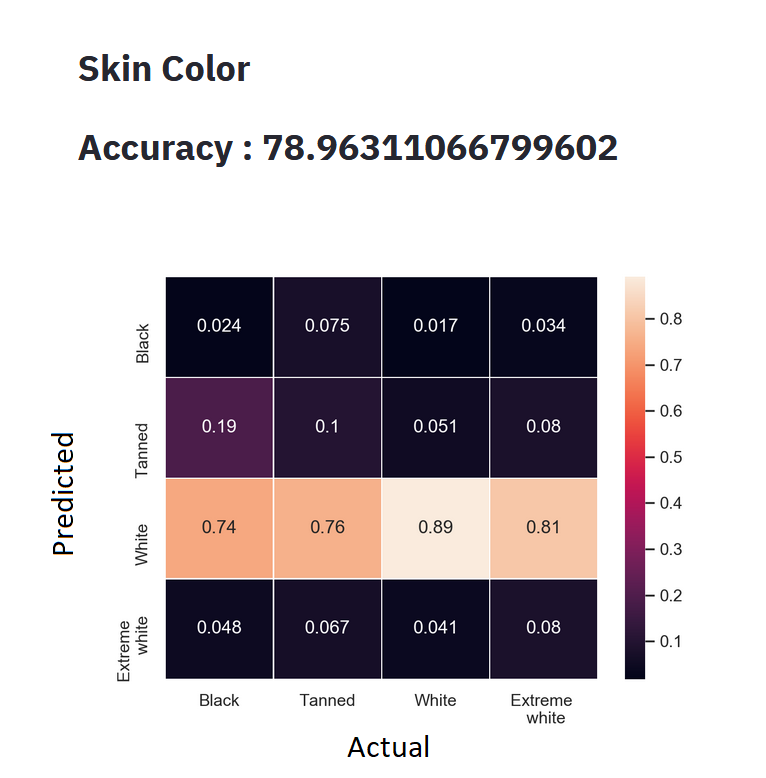
\includegraphics[width=0.65\textwidth]{images/skin_lock_color.png}
\caption{Skin color confusion matrix.}
\centering
\label{fig:skin_lock_color}
\end{figure}


\subsubsection{Skin Texture}
Figure \ref{fig:skin_lock_texture} displays the confusion matrix of the skin texture characteristic. While having an average accuracy, the model seems to predict young-plus more times than the others. When the model tries to predict the class for an image that has an actual texture of young, adult or aged, it confuses it with young-plus in more than 50\% of the images. Once again, here we have the same problem as in some other characteristics, the amount of samples from the classes in the dataset is not uniform as we see in table \ref{tab:skin_text}.

\begin{figure}[H]
\centering 
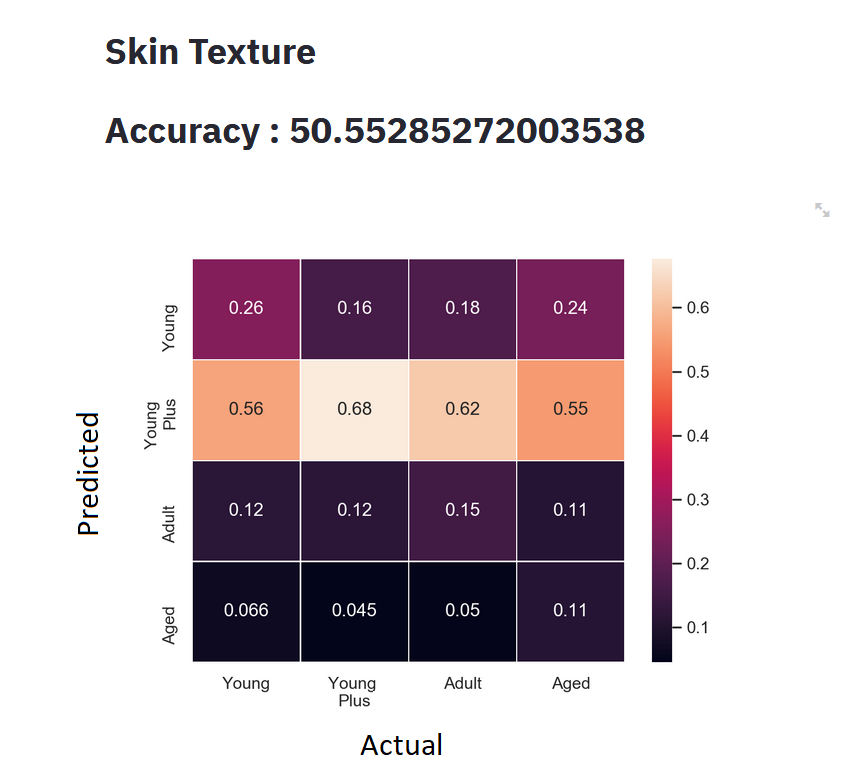
\includegraphics[width=0.65\textwidth]{images/skin_lock_texture.png}
\caption{Skin texture confusion matrix.}
\centering
\label{fig:skin_lock_texture}
\end{figure}

\subsubsection{Spots}
Figure \ref{fig:spots_lock} displays the confusion matrix of the spots characteristic. This 
characteristic has an average overall accuracy but the model seems to predict a lot more 0 spots than the others. By analysing table \ref{tab:spots} together with this matrix, we notice that this is due to the fact that there are around 8000 samples images with 0 spots and the amount of samples with other classes is not even half of that. Due to this, the model doesn't learn how to recognize the other classes and tends to only predict 0 spots.
\ref{tab:spots}

\begin{figure}[H]
\centering
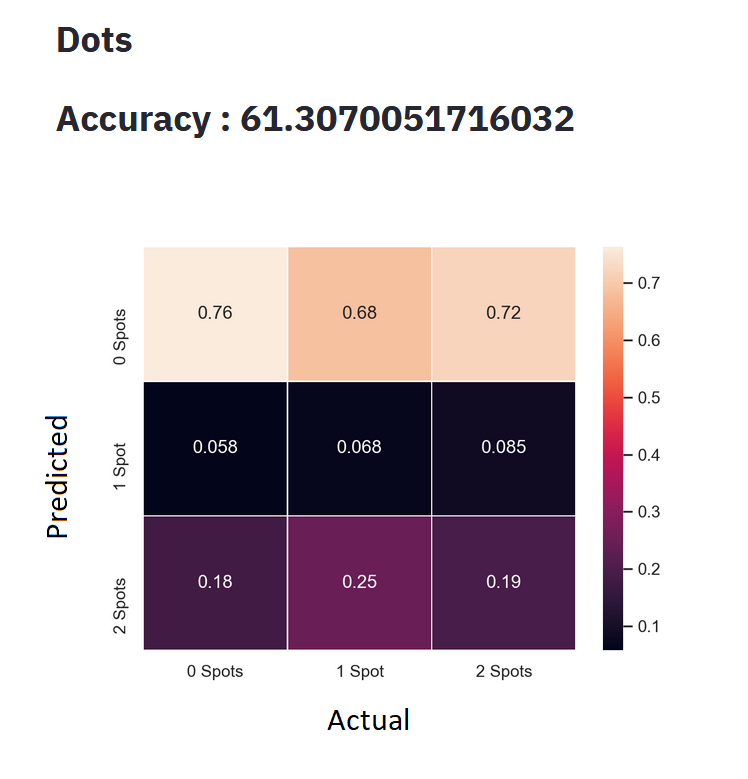
\includegraphics[width=0.65\textwidth]{images/dots_lock.png}
\caption{Spots confusion matrix.}
\centering
\label{fig:spots_lock}
\end{figure}





\subsubsection{Discussion}
Confusion matrices are one of the best ways to analyse the discriminator model in depth. Just by analysing each one of these matrices we get all this crucial information about the percentage of times that the model predicts correctly a certain class and also the times where it outputs a wrong prediction. With this data we can figure the current errors in the model and try to implement solutions.




\par

I believe that the biggest problem that leads to the results shown in subsection \ref{ssec:highm}, is the lack of consistency in the dataset. The fact that the model is trained with different sample sizes of certain classes makes it so that the model doesn't learn equally to distinguish some of them, and as a result, we have these predictions where the model only tends to predict a certain class because it has not learned how to recognize the rest.


\par

Something to also have in mind during the experiments in this section is the fact that, as mentioned in subsection \ref{sub:brute} and in subsection \ref{sub:safe}, we are comparing the actual combinations of an image with the combination that got the best probability according to the discriminator. As a result, in these cases, there are going to be wrongly predicted characteristics. In a perfect scenario these would be the best results possible, where the discriminator always outputs the highest probability to the actual combination of an image, but this model is not perfect and because of that there are going to be a lot of cases where we can't always take in consideration the combinations with the highest probability. In order to minimize this problem I implemented the A* algorithm, which we will see in subsection \ref{ss:astar}, produced better results by taking this problem in consideration.


\subsection{A* Algorithm}
\label{ss:astar}
As we saw in subsection \ref{ssec:highm} the fact that these last algorithms did not take in consideration that the actual combination does not always have the highest probability according to the discriminator, led to prediction errors in some of the characteristics.  

\par
When using the A* algorithm the estimated time to get the best fitting combination to an image is between 1 and 20 seconds. This interval is due to the way that the A* algorithm is implemented, as mentioned in //Secção de impleentação do Aestrela// the algorithm starts in a random combination and from there it starts to analyse the following combinations, after calculating the best successor, the algorithm repeats the process for the chosen combination to follow. As a result, since the starting combination is random, the algorithm can get lucky and start on a combination that already has similarities with the image or it can get unlucky and start on a combination that doesn't match the image at all, and thus, taking more time to find it's way to the best combination.

\subsubsection{Discussion}
From my perspective this algorithm is efficient, and since it takes in consideration the fact that the discriminator is not perfect, it is the best fit for this system. The implementation of this algorithm not only helps in efficiency but will also scale with the system, meaning that, if more characteristics are added and the number of possible combinations increases, this algorithm will be able to still find the desired combination and in a reasonable amount of time. In subsection \ref{ss:astaralg} we will analyse what impact this algorithm has on the results.

\subsection{A* Algorithm Confusion Matrices}
\label{ss:astaralg}
After implementing the A* algorithm and using it for all the test images I decided to also generate confusion matrices to analyse if the results were better or worse than with the other algorithms. 
\par
For each matrix represented in this section I will be comparing it to the respective matrix using the other algorithms, so it is easier to draw some conclusions about which ones fit the best for this system.


\subsubsection{Eyebrow Distribution}
Figure \ref{fig:eybrows_star_distr} displays the confusion matrix of the eyebrow distribution characteristic. The first detail we notice when analysing this matrix is that the overall accuracy of the model towards this characteristic is 63.7\%, which is significantly higher than the overall accuracy obtained with the other algorithms. 


\par

This is also reflected in the diagonal entries, for instance, when the images had an actual average distribution the model correctly predicted it 74\% of the times which is also an improvement from the results we had before. The other two classes also got accuracy improvements, when the images had an actual sparse distribution, the model correctly predicted it in 22\% of the images and likewise when images had an actual dense distribution the model correctly predicted it in 47\% images.    


\begin{figure}[H]
\centering
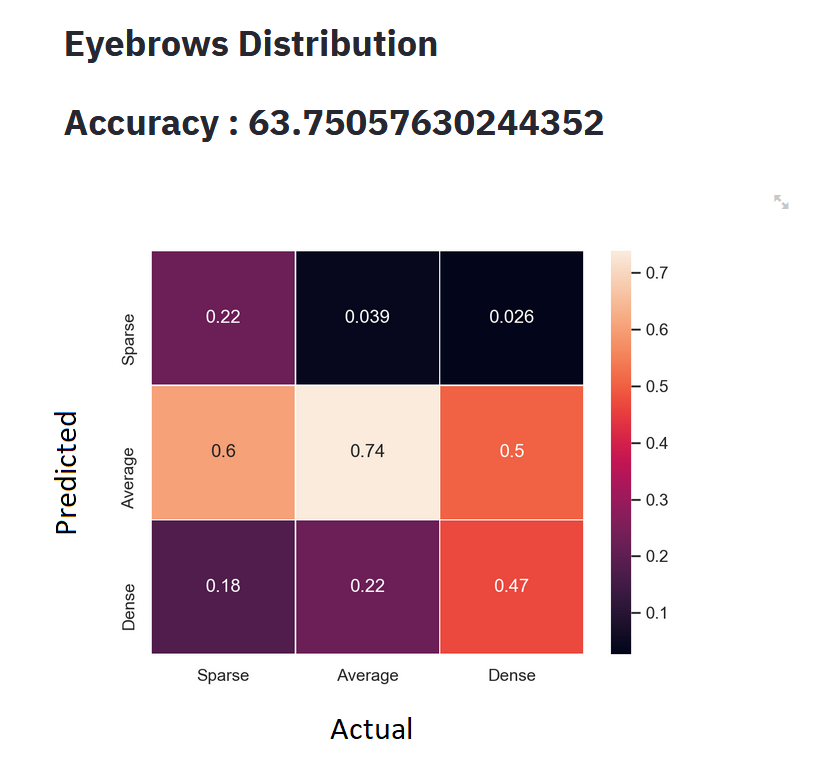
\includegraphics[width=0.65\textwidth]{images/eyebrows_star_distribution.png}
\caption{Eyebrow distribution confusion matrix.}
\centering
\label{fig:eybrows_star_distr}
\end{figure}


\subsubsection{Eyebrow Shape}
Figure \ref{fig:eybrows_star_shape} displays the confusion matrix of the eyebrow shape characteristic. When it comes to this characteristic, the model still tends to predict round most of the times. Although, by using the A* algorithm it improved the overall accuracy of the model for this characteristic, especially when the image had an actual round shape the model correctly predicted it 55\% of the times, which is an improvement from the 49\% from the previous algorithms.



\begin{figure}[H]
\centering
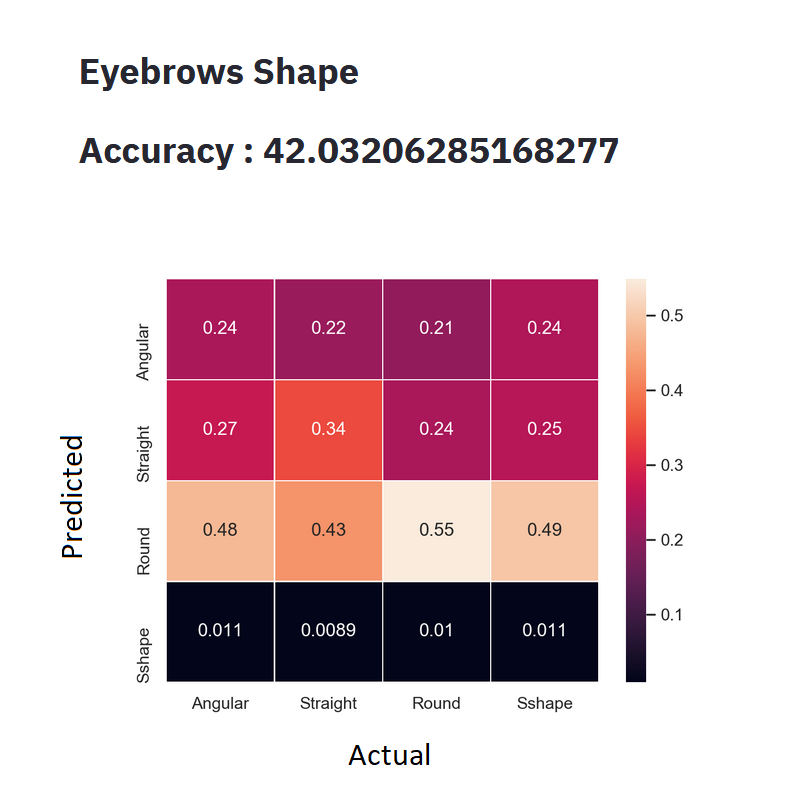
\includegraphics[width=0.65\textwidth]{images/eyebrows_star_shape.png}
\caption{Eyebrow shape confusion matrix.}
\centering
\label{fig:eybrows_star_shape}
\end{figure}



\subsubsection{Eyebrow Size}
Figure \ref{fig:eybrows_star_size} displays the confusion matrix of the eyebrow size characteristic. In comparison with figure \ref{fig:eyebrow_lock_size}, we notice that even though the overall accuracy did not increase a significant amount, there is an improvement of accuracy in terms of individual classes. For instance, when an image has a small eyebrow size the model correctly predicted it 45\% of the times which is better compared to the 25\% accuracy using the other algorithms. 

\par

Despite the fact that there was improvements on certain classes, medium size suffered a downgrade on accuracy since the model only correctly predicted 36\% of the times compared to the 44\% accuracy using other algorithms.

\par

Something to take in consideration is that while using the other algorithms the results were heavily influenced by medium and large size, although, in this matrix we see that the predictions are a lot more uniform and also predicting small size.



\begin{figure}[H]
\centering
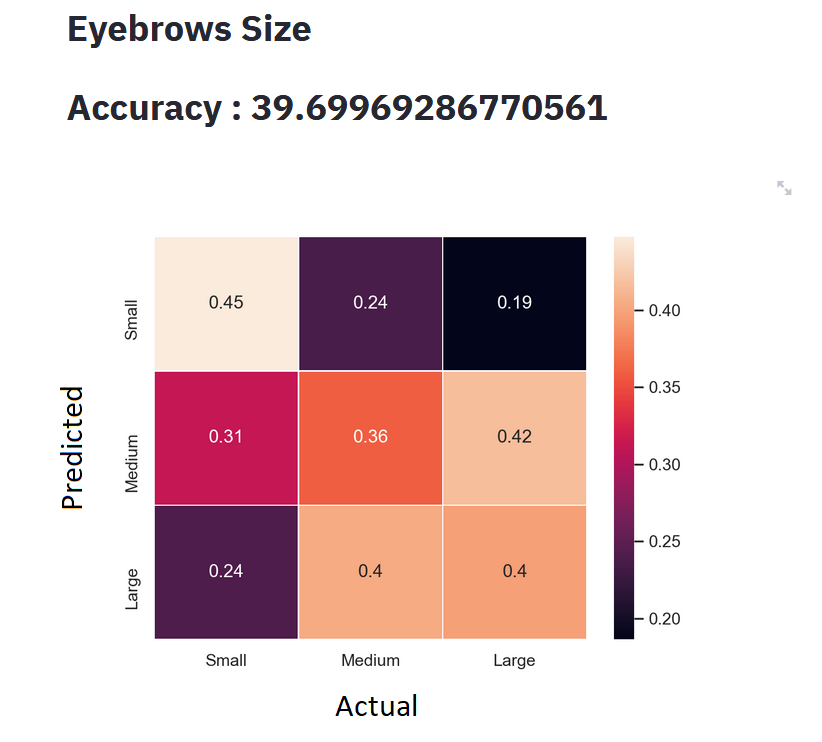
\includegraphics[width=0.65\textwidth]{images/eyebrows_star_size.png}
\caption{Eyebrow size confusion matrix.}
\centering
\label{fig:eybrows_star_size}
\end{figure}


\subsubsection{Eyelashes Size}
Figure \ref{fig:eyelashes_star_size} displays the confusion matrix of the eyelashes size characteristic. When comparing the matrix to the one in figure \ref{fig:eyelashes_lock_size}, we see that the overall accuracy improved, and we also notice that using this algorithm we get more variety of predicted classes, since using the other algorithms the predictions were highly on class 1.  

\par


The fact that class 2 still does not get predicted correctly most of the times is, once again, due to the fact that the amount of samples of that class in the dataset is small compared to the others.

\begin{figure}[H]
\centering
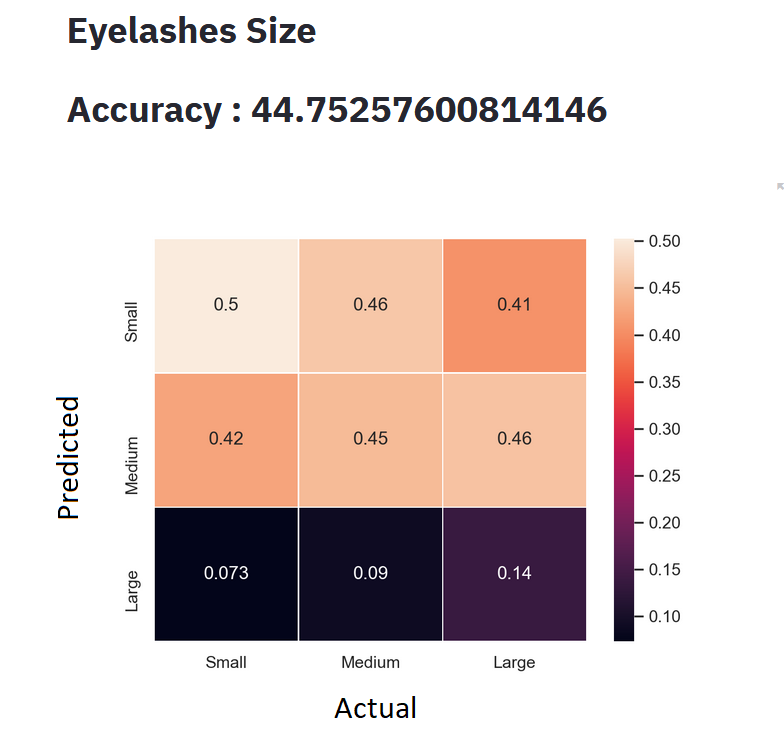
\includegraphics[width=0.65\textwidth]{images/eyelashes_star_size.png}
\caption{Eyelashes size confusion matrix.}
\centering
\label{fig:eyelashes_star_size}
\end{figure}


\subsubsection{Eyelids Shape}
Figure \ref{fig:eyelids_star_shape} displays the confusion matrix of the eyelids shape characteristic. In this matrix we notice that there is some confusion between the two classes, although, when in figure \ref{fig:eyelids_lock_shape} we could see that fall was the most predicted, by using this algorithm we notice that there is a more even distribution on correct predictions and not only focused on the fall shape.


\begin{figure}[H]
\centering
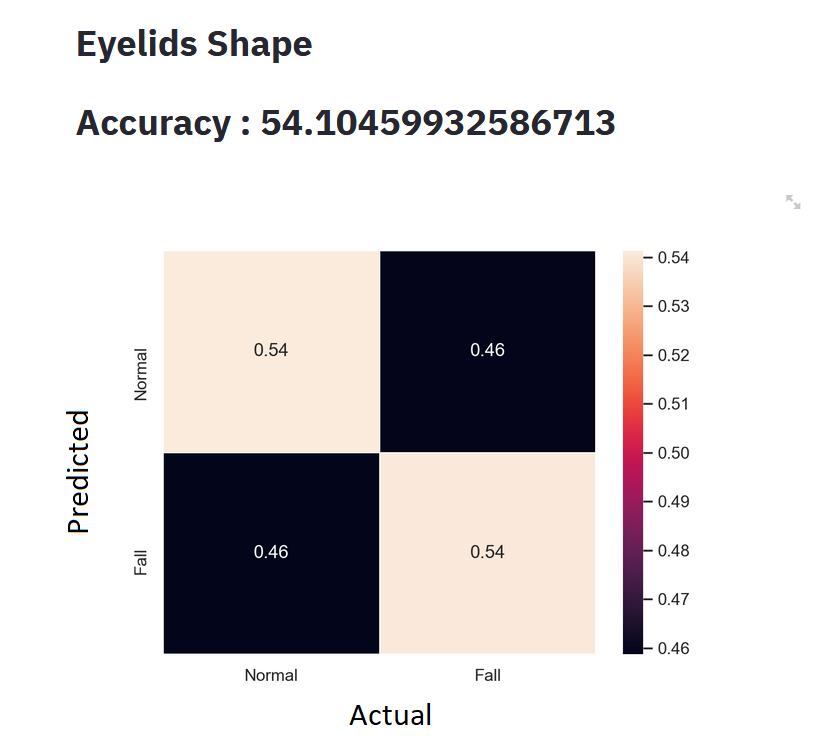
\includegraphics[width=0.65\textwidth]{images/eyelids_star_shape.png}
\caption{Eyelids shape confusion matrix.}
\centering
\label{fig:eyelids_star_shape}
\end{figure}



\subsubsection{Iris Color}
Figure \ref{fig:eyelids_star_shape} displays the confusion matrix of the eyelids shape characteristic. This is one of the characteristics that benefit the most with the A* algorithm. The reason behind this, is that, since the dataset does not have nearly the same amount of samples for each class, the model does not learn how to recognize the classes in minority, and thus, the combinations with the highest probability will be the ones that do not contain these characteristics. This is where the A* algorithm comes in handy, by not focusing on the combinations with the highest probability, it outputs combinations that are more accurate. 


\par

For instance we can see that previously in the matrix represented in figure \ref{fig:Iris_lock_color}, whenever the actual eye color was blue the model only predicted it correctly 15\% of the times. However, when we take in consideration the discriminator's error with the A* algorithm, we see a huge improvement on the percentage of correct predictions for this class.


\begin{figure}[H]
\centering
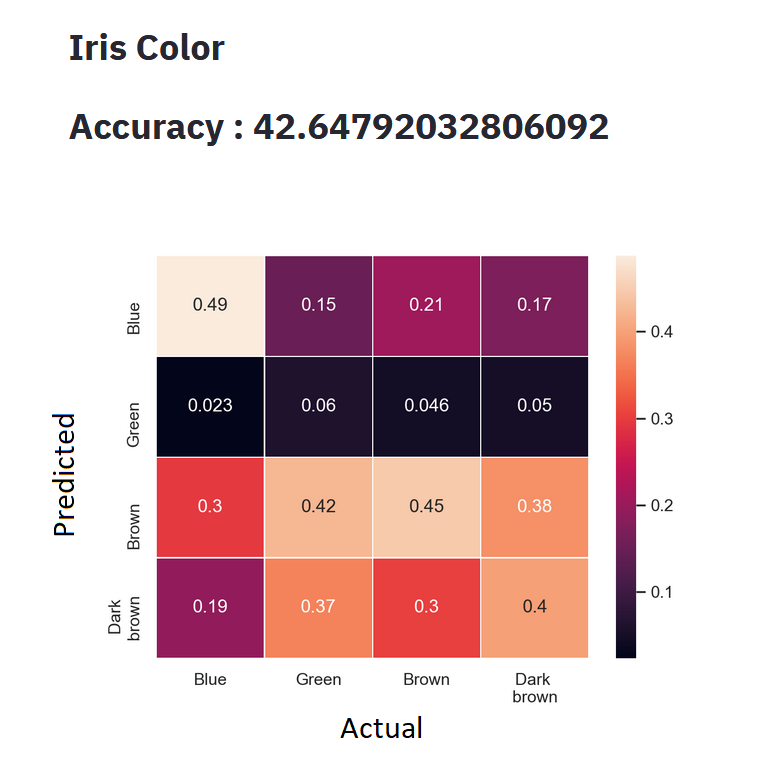
\includegraphics[width=0.65\textwidth]{images/iris_star_color.png}
\caption{Iris color confusion matrix.}
\centering
\label{fig:iris_star_color}
\end{figure}


\subsubsection{Skin Color}
Figure \ref{fig:skin_star_color} displays the confusion matrix of the skin color characteristic. Despite the overall accuracy being lower using the A* algorithm, we have to take into account that the dataset has a huge discrepancy when it comes to the class samples of this characteristic, which leads to the high tendency of the model to predict the white color. Although, when using the A* algorithm, we notice some improvements on the other colors, for instance, the black color which had a 2.4\% accuracy now has a 15\% accuracy. This is also the case for extreme white color, which had a previous accuracy of 8\% and now has an accuracy of 16\%.  


\begin{figure}[H]
\centering
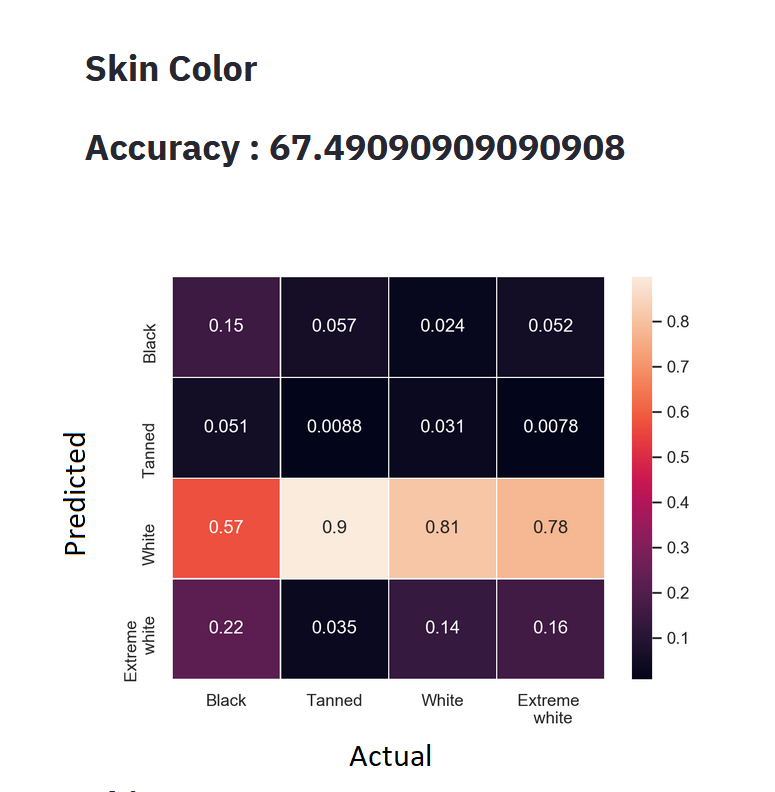
\includegraphics[width=0.65\textwidth]{images/skin_star_color.png}
\caption{Skin color confusion matrix.}
\centering
\label{fig:skin_star_color}
\end{figure}



\subsubsection{Skin Texture}
Figure \ref{fig:skin_star_texture} displays the confusion matrix of the skin color characteristic. Just like in the previous characteristics, in this matrix we notice that there is a more variety of predictions instead of them all being concentrated into one class. 

\par

The matrix represented in figure \ref{fig:skin_lock_texture} shows that when using other algorithms the predictions were all focused on young-plus, although, when we use the A* algorithm we see that young, adult, and aged get improvements on their accuracy. For instance, when previously when the actual texture of an image was young the model would correctly predict it 26\% of the times, now the model correctly predicted it 54\% of the images. This is also noticeable for the adult and aged classes, that previously had 15\% and 11\% respectively and now have 20\% and 15\%. 

\begin{figure}[H]
\centering
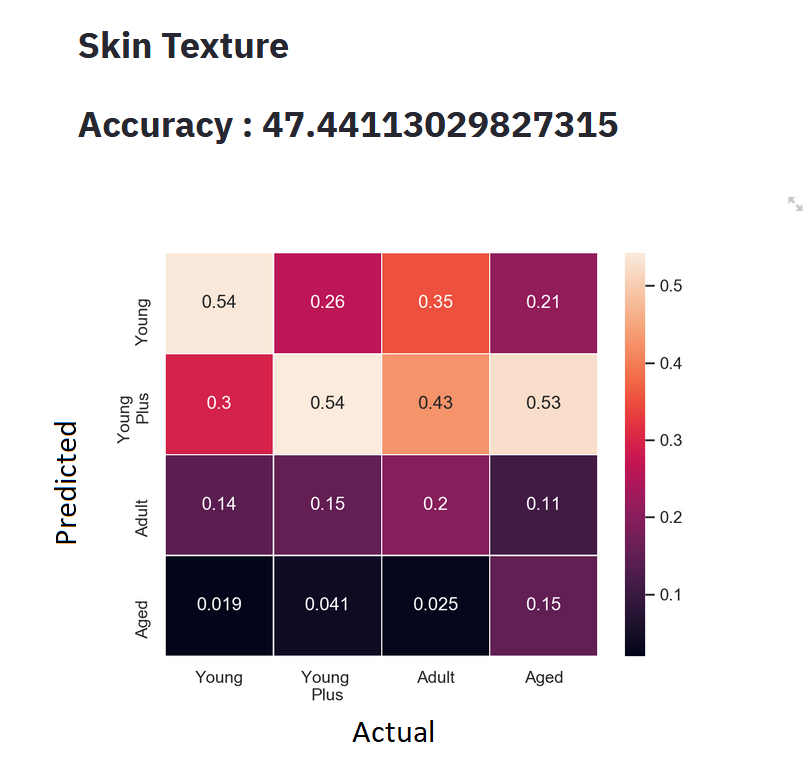
\includegraphics[width=0.65\textwidth]{images/skin_star_texture.png}
\caption{Skin texture confusion matrix.}
\centering
\label{fig:skin_star_texture}
\end{figure}



\subsubsection{Spots}
Figure \ref{fig:dots} displays the confusion matrix of the skin color characteristic. In this matrix we notice that there was an accuracy improvement for 0 spots, and logically, due to the fact that the dataset being so unbalanced, this is the only improvement possible.

\begin{figure}[H]
\centering
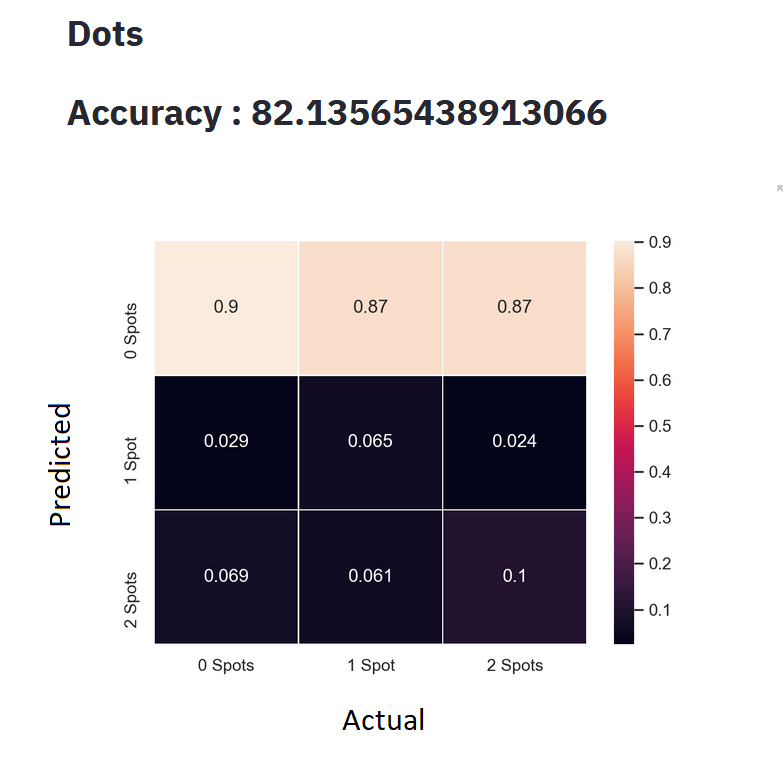
\includegraphics[width=0.65\textwidth]{images/dots_star.png}
\caption{Spots confusion matrix.}
\centering
\label{fig:dots}
\end{figure}

\subsubsection{Discussion}
From my perspective the A* algorithm is not only an efficient way of finding the best combination to a given image, but is also the best algorithm to take in consideration the discriminator's mistakes. 

\par
Based on the results shown in subsection \ref{ss:astaralg} we notice that the discriminator is indeed focusing on some classes more than others. This mistake is clearly due to the unbalanced number of samples of some classes, for an instance, the characteristic that suffers mostly from this, as we see in table \ref{tab:skincolor}, is the skin color characteristic. Due to this, there are classes that the discriminator is not going to be able to recognize and thus, leading to the combinations with the highest probability not always being the correct ones as explained before. This is a problem that would only be solved if we had a balanced dataset and a perfectly trained model. With this being said, the A* is well suited for this system because it takes these mistakes in consideration and the system will always have margins of error. As mentioned in section // REFERIR SECÇÃO DE IMPEMENTACAO A*// we can always change the average probability that the algorithm will be looking for while searching for the best fitting combination. 


\par

The downside of this algorithm is that, if the correct combination is the highest combination possible, the algorithm will probably miss it. But, since these cases do not happen that often, it does not justify not implementing this algorithm in the system.


\section{Classification Algorithms Experiments}
\subsection{\acs{MLP} Experiments}
Being such a simple model, the amount of experiments needed to achieve an high accuracy were not many. The only variable that I experimented with was the amount of hidden layers on the model. After some experimentations at adding layers to the model, there were not any significant changes it's accuracy and thus, the final implementation of this model only has two hidden layers as observed in figure \ref{label}. When it comes to the accuracy of the model, the highest value obtained on the test dataset was 98\%. Figure \ref{fig:loss_mlp} represents the loss of the model during training, and since the accuracy has an inverted correlation with the accuracy, we can see that the loss also was minimized to 0.02. // BEtter values for loss and accracy





\begin{figure}[H]
	\centering
	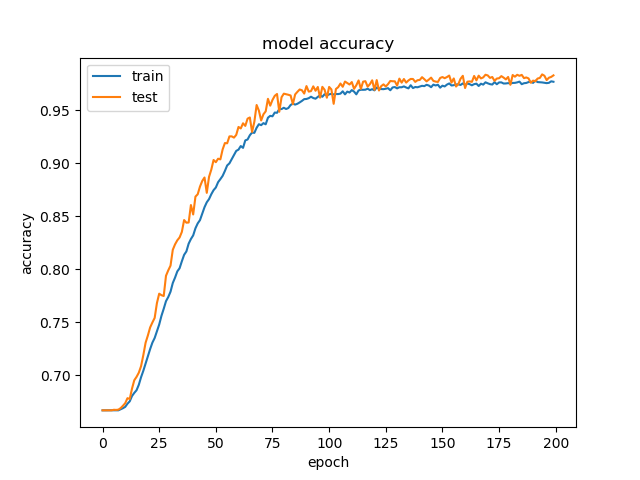
\includegraphics[width=0.65\textwidth]{images/accuracy_mlp.png}
	\caption{\acs{MLP} training accuracy.}
	\centering
	\label{fig:accuracy_mlp}
\end{figure}

\subsubsection{Discussion}
This system can benefit a lot from the implementation of this model since it's accuracy is excellent. With this being said, the model lacks interpretability, which is the whole purpose of this project. As we will see in subsection \ref{sub:C4.5}, the C4.5 algorithm will be worse when it comes to accuracy but it is more interpretable and easy to know why the model took a certain decision.


\subsection{\acs{C4.5} Experiments}
\label{sub:C4.5}
The first data we get from training the C4.5 algorithm is the \textbf{Feature Importance}, shown in figure \ref{label}. This table indicates how much a feature is taken in consideration when making decisions. Compared to the \acs{MLP} this is already a great improvement when it comes to interpretability. Another feature that makes this algorithm perfect for this system is the fact that we can literally visualise the decision tree that was generated by the algorithm and analyse how it makes its decisions.


 \par
 
 When it comes to acccuracy the model tends to perform worse than the \acs{MLP} model, with 75\% accuracy on the testing set. But, since it is not a bad accuracy overall, it does not override the fact that the model is much more suitable for a system like this due to its amazing interpretability.


\begin{figure}[H]
	\centering
	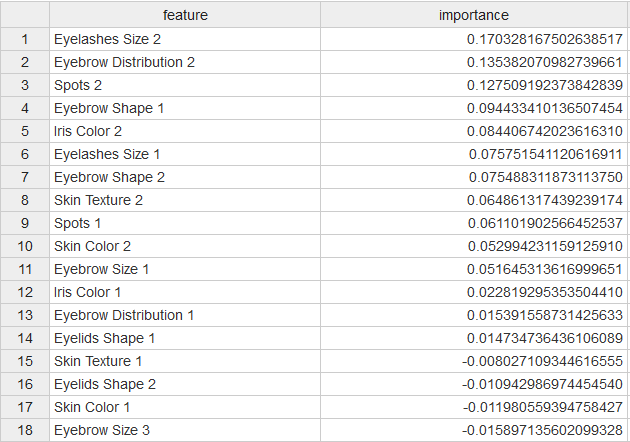
\includegraphics[width=0.65\textwidth]{images/FeatureImportance.png}
	\caption{Feature Importance data.}
	\centering
	\label{fig:accuracy_mlp}
\end{figure}

\subsubsection{Discussion}
In my perspective, the decision tree generated by the C4.5 algorithm is a great implementation to this system. As stated before, eventhough the \acs{MLP} model has a better accuracy than the decision tree, it does not override the fact that a decision tree is so much more interpretable than a neural network. Just by analysing the \textbf{Feature Importance} table, we get crucial information about features and the consideration that the model has for each one of them, using this information, we too can make decisions, for instance, if a feature brings zero value for the model's decision, maybe it could be removed or replaced by another one more significant.

\par

I believe that interpretabity is the key factor is systems like this one, it allows us to make rational decisions instead of changing parameters and hoping for the best. Instead, we can analyse what is taken in consideration by these models and use that information to improve the system overall. Also, eventhough the \acs{MLP} model has an excellent accuracy now, if in any future implementations more characteristics are added to this system and the it performs worse, we can not know for sure which characteristics are making it lose performance and which ones are valuable to the system overall. This is not the case for the decision tree model, if there were new characteristics added to the system, it would be able to explain which ones are degrading the system and which ones are actually valuable to it.



\clearpage{\thispagestyle{empty}\cleardoublepage}

\chapter{Conclusions and Future Work}

\section{Main Conclusions}

\section{Future Work}


\clearpage{\thispagestyle{empty}\cleardoublepage}

% SE EXISTIREM APENDICES, DESCOMENTAR O QUE ESTÁ EM BAIXO
% \appendix
% \include{apendice1}
% \clearpage{\pagestyle{empty}\cleardoublepage}
% \include{continuacao}
% \clearpage{\pagestyle{empty}\cleardoublepage}
% \include{apendice2}
% \clearpage{\pagestyle{empty}\cleardoublepage}
% \include{apendice3}
% \clearpage{\pagestyle{empty}\cleardoublepage}

\backmatter

\bibliographystyle{plain}
\bibliography{bibliografia}

\end{document}